\documentclass[a4paper]{profusion}

\usepackage{verbatim}
\usepackage{graphicx}
\usepackage{color}

\newcommand{\GUICheckbox}[1]{\textcolor{red}{#1}}
\newcommand{\GUIButton}[1]{\textcolor{green}{#1}} % buttons and list items
\newcommand{\GUIIcon}[1]{\textcolor{blue}{#1}}    % buttons with no
                                                  % visual feedback on
                                                  % mouse click
\newcommand{\GUILabel}[1]{\textcolor{magenta}{#1}}
\newcommand{\GUIEditable}[1]{\textcolor{yellow}{#1}} % Text entries,
                                                     % pop-up lists,
                                                     % etc

\title{Editje\\
  \normalsize{User's manual}}

\ProFUSIONMail{\{glima,ivan,tiago\}@profusion.mobi}
\author{Gustavo Lima Chaves \hspace{1cm} Iván Briano \hspace{1cm}
  Tiago Rezende Campos Falcão}

\begin{document}

\maketitle
\tableofcontents
\listoffigures

\section{Introduction}

Editje is a ``what you see is what you get'' tool for creation of
graphical user interfaces for applications which use the Edje
library. It is an alternative to the ``usual'' way of accomplishing
this task, which is by editing \texttt{.edc} text files and compiling
them into \texttt{.edj} ones.

Editje can open and edit both \texttt{.edc} and \texttt{.edj} forms of
interface declarations, saving them back in the form they were opened
with.

This document describes briefly Editje's features and functionality.
%TODO: also document the installation steps, later

\section{Opening a File}

Editje's invoking command, if you're using a terminal to launch it, is
\texttt{editje-bin}. If invoked like that, with no arguments, it will
show the screen pictured in figure \ref{fig:open_file}.

\begin{figure}[h!]
  \centering
  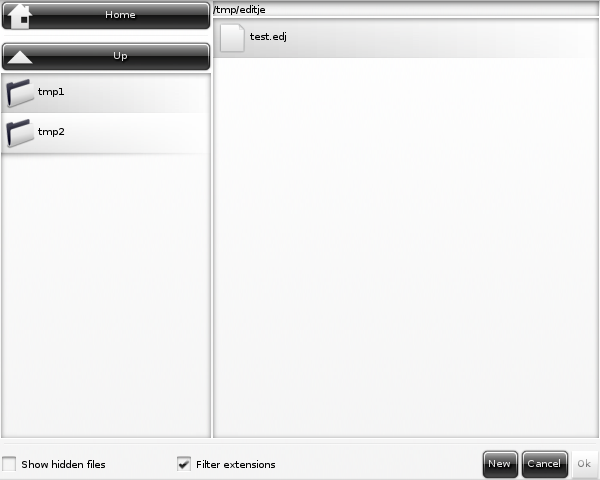
\includegraphics[width=0.87\textwidth]{images/open_file.png}
  \caption{``Open file'' dialog}
  \label{fig:open_file}
\end{figure}

The actions on that window are straightforward: you navigate through
directories on the list on the left side and select files to open on
the files list, on the right. The latter list shows the files in the
current folder, which was selected on the former one. The
\GUICheckbox{``filter extensions''} checkbox will only list files
whose extension match \texttt{.edc} or \texttt{.edj}.

%FIXME: the fscking \times, instead of 'x' (not working)
If a (valid) file on the list on the right is selected, you may click
the \GUIButton{``Ok''} button and Editje will open it and lead you to
its main window. The \GUIButton{``New''} button will ask you for a
name to a \emph{new} file to work on. Just give it a name and hit
\GUIButton{``Ok''} to start editing it. To the current date, this new
file starts with just one group, named ``main'', with no parts and
with a default size of 500x500 pixels. Group templates will come as an
option to start new files, shortly.

%% Editje may also be invoked with one or two arguments, which are,
%% respectively:
%% \begin{itemize}
%%   \item path to file to open and
%%   \item name of a group, in that edje file, to edit.
%% \end{itemize}

Editje may also be invoked with one argument, which is the path to a
file to open. Whether you choose a file in the dialog shown in figure
\ref{fig:open_file} or by giving its path in the command line, you'll
get a dialog box asking for a group to edit, between the ones Editje
finds inside the chosen file (see figure \ref{fig:choose_group}).

%FIXME: bad pic! we gotta fix the centering issue asap
\begin{figure}[h!]
  \centering
  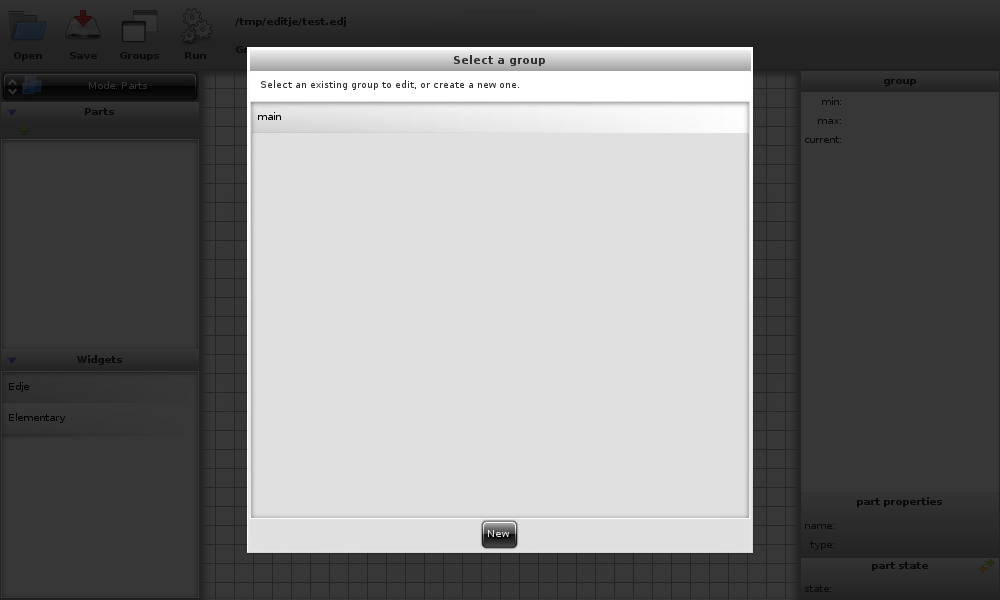
\includegraphics[width=1.0\textwidth]{images/choose_group.png}
  \caption{Group choice dialog}
  \label{fig:choose_group}
\end{figure}

As you see, in that box you have a list of the group names found in
the file. When one of the list items is selected, the respective group
will have a \emph{preview image} shown on another page of the group
choice dialog (figure \ref{fig:group_preview}). Click on
\GUIButton{``Open''} if you're sure you want to start editing this
specific group. \GUIButton{``Cancel''} will lead you back to the page
shown in figure \ref{fig:choose_group} and \GUIButton{``Delete''},
naturally, will remove that group from the file's group
collection\footnote{It will refuse to delete all groups from a file,
  though.}.

\begin{figure}[h!]
  \centering
  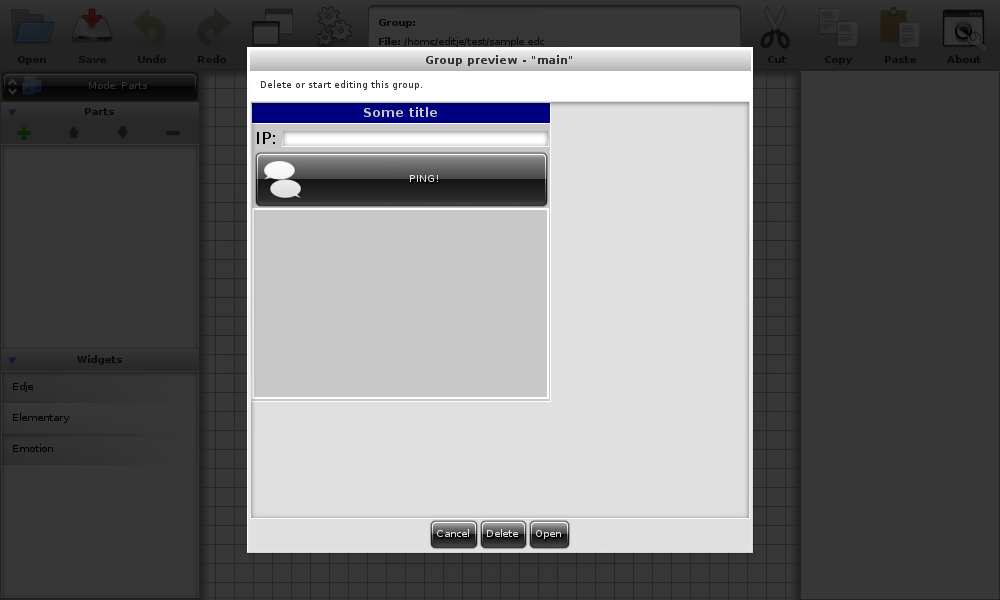
\includegraphics[width=1.0\textwidth]{images/group_preview.png}
  \caption{Group choice dialog: group preview}
  \label{fig:group_preview}
\end{figure}

Finally, there's the button \GUIButton{``New''}, found in this
dialog's first page. As you may imagine, it's going to lead you to a
third page, asking for a name to the group to be created. From there,
you may desist and go back one page or, if sure, create and start
editing the fresh new group. This group will also be 500x500 sized and
have no parts.

\section{Editje's Window}

Once you open a file, you'll reach Editje's main window, which is
depicted on figure \ref{fig:main_window}.

% - program used to draw the overlaying objects: Kolourpaint
% - font used to overlay numbers: Free Sans, 52
\begin{figure}[h!]
  \centering
  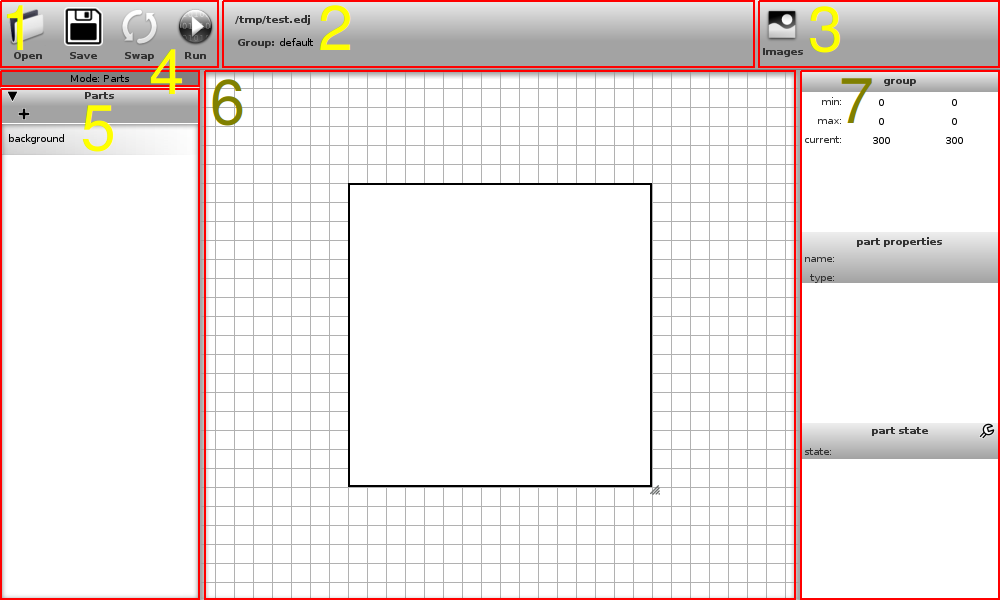
\includegraphics[width=1.0\textwidth]{images/main_window.png}
  \caption{The main window}
  \label{fig:main_window}
\end{figure}

Each of its \emph{main interacting areas} were marked with red
rectangles and numbered. The following is a description of each of
them:

\begin{description}
\item[1 -- Actions on file and group]
  The first action, \GUIIcon{``Open''}, will call the same dialog
  window you saw if you called Editje with no arguments. When you
  select the file to operate on, you'll get \emph{another} independent
  instance of a main window with an opened file. It's \emph{not}
  another instance of the editor, though, and the process will only
  finish when the last editor's window is closed.

  The second action, \GUIIcon{``Save''}, naturally tells the editor to
  save back the modifications on the file under edition. As said
  before, they get saved in the same format they were opened with, be
  it \texttt{.edc} or \texttt{.edj}.

  The \GUIIcon{``Groups''} one will raise the same box you get when
  calling Editje with just a file name argument -- the group selection
  box (figure \ref{fig:choose_group}). Those same actions will be
  available, here. Note that, if you select another group to edit, at
  this stage it \emph{won't} ask if you want to save the modifications
  on the group being left, so make sure you have them saved before
  switching groups.

  Finally, there's the \GUIIcon{``Run''} action. It will open a window
  with a \emph{live} version of the group being edited. You'll be
  able, then, to interact with it and test its behavior for user input
  events. Just close that window to get back to normal edition.

\item[2 -- File and group names] On the bottom of this area you'll see
  the full path to the file being edited. On the top, after the label
  \GUILabel{``Group:''}, you see the name of the group under
  edition. You may change the group's name by editing it directly:
  it's a text entry. Just hit the return key after you're done and the
  change will get applied.

\item[3 -- Mode dependent actions] This region of the main screen is
  populated with action icons accordingly to the \emph{mode} Editje is
  working on (see region 4, which follows). For the initial
  (``Parts'') mode, this region presents an icon which, when clicked,
  will raise a box with author and licensing information of the edje
  editor itself.

\item[4 -- Mode selection] Editje has \emph{three} modes in which it
  operates:
  \begin{itemize}
  \item Parts
  \item Animations
  \item Signals
  \end{itemize}
  When you start it, you'll be in the first one. This is the mode in
  which you create and edit parts. The other two, respectively, are
  the modes in which one creates and edits animations and signals. The
  actions available for each mode are going to be described
  incrementally. If you want to change the mode of operation, just
  click on the button surrounded by this region and select the desired
  mode.

\item[5 -- The group displaying (and manipulation) area] This is where
  you actually \emph{see} the effects of your editions on a group and
  its parts. The group boundaries are marked by the thick black lines
  forming a rectangle and with the symbol seen in figure
  \ref{fig:group_edje}, at the bottom right corner. This happens to be
  also the icon that, when clicked over and moved, will resize the
  whole group. More on part manipulation will be addressed on section
  \ref{sec:part_editing}.

\begin{figure}[h!]
  \centering
  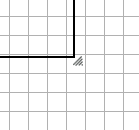
\includegraphics[width=0.2\textwidth]{images/group_edje.png}
  \caption{Group resizing knob}
  \label{fig:group_edje}
\end{figure}

\item[6 -- Group and selected part properties] This is the region on
  the interface where the user will be able to \emph{see and edit} the
  properties of the group being edited and the selected part, if any
  is selected. There are three collapsable groups of properties
  there. You can show/hide them by clicking over their title labels,
  which are:

  \begin{description}
    \item[\GUILabel{``group''}] properties of the group being edited
    \item[\GUILabel{``part properties''}] properties of the currently
      selected part, if any
    \item[\GUILabel{``part state''}] properties of the current
      \emph{state} under edition of the selected part
  \end{description}

For each of them, if the user sees only the title on the interface, it
means that that group of properties is \emph{collapsed}. Just click
over this title and it will get expanded. These interface groups will
be described better on section \ref{sec:part_editing}.

\item[7 -- Parts list] This is, while in ``Parts'' mode, an area which
  lists all the parts composing the group being edited and has also
  some actions on them. These actions will be described better later
  in the document. On the bottom of this area, one sees the \emph{list
    of available widgets/parts}. From this place, you'll see all types
  of GUI elements Editje supports. Interaction with this list is one
  the ways of telling the editor to add new widgets to the group under
  edition.

\end{description}

\section{Basic Part Editing}
\label{sec:part_editing}

Visual editing of an edje interface begins with part handling, which
is done under the ``Parts'' mode. In this mode, the user is able to
add and edit parts in the current group, setting all of their
available properties. Part states can also be created and edited while
in this mode.

\subsection{Adding and selecting parts}

 We start with the part addition feature, which is accessible through
 the \GUIIcon{``+''} icon on region 3 of figure
 \ref{fig:main_window}. Once you click there, you get a dialog box
 like the one shown in figure \ref{fig:add_part_box}.

\begin{figure}[h!]
  \centering
  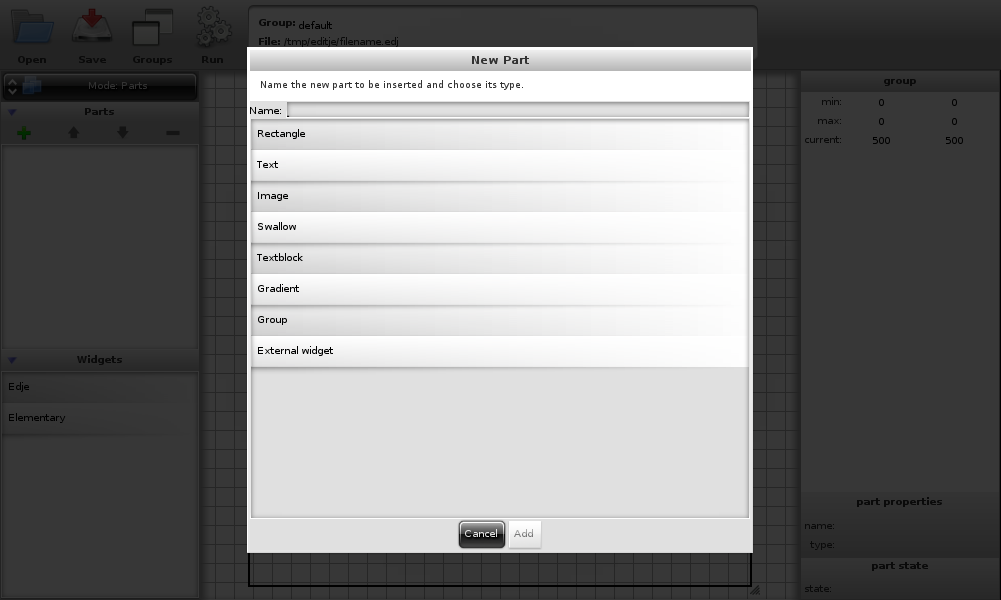
\includegraphics[width=1.0\textwidth]{images/add_part.png}
  \caption{``New Part'' dialog}
  \label{fig:add_part_box}
\end{figure}

Clicking over any of the list entries will select that given
\emph{type} to the part being added and give a default name to it,
appearing in the text entry on the top. You may edit that name as you
wish\footnote{Editje will complain only if that name belongs to
  another part already present on the group under edition.}. The
``External Widget'' type is special: it's a meta type which will let
you select objects from external modules (exporting edje objects) as
parts of your interface. Currently, the only module supported is
Elementary, a widget library which has some of its widgets with
properties externalized to edje-edition.

Then, if you click over \GUIButton{``External Widget''}, the bottom
part of the dialog box will show two lists side-by-side. The left one
lists the modules exporting widgets for edje-edition, while the right
one lists the actual widgets for the module selected on the left.

Accordingly to figure \ref{fig:add_part_box}, Editje has the following
supported types of parts:

\begin{itemize}
  \item rectangle,
  \item text,
  \item textblock,
  \item image,
  \item gradient,
  \item swallow,
  \item group and
  \item external widget.
\end{itemize}

If, when adding a new part, you choose the rectangle type, you'll end
with a new object similar to the one seen on figure
\ref{fig:new_rectangle}, whose name is, in our context,
``\texttt{Rectangle01}''. Screen regions of interest have been
numbered, in that figure. If you look at region 3, the parts list,
you'll see it populated with our new part.

\begin{figure}[h!]
  \centering
  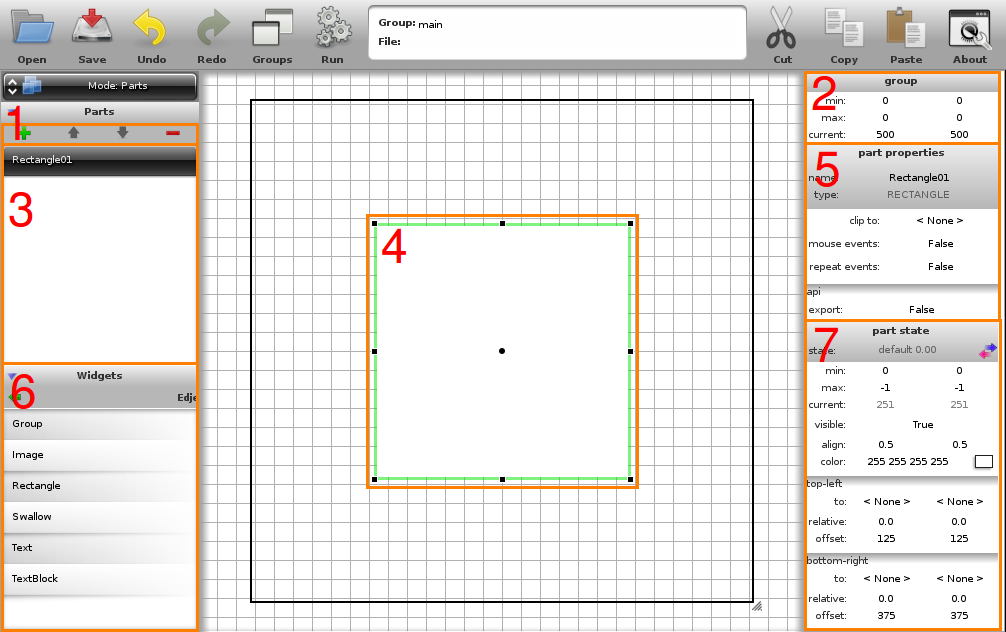
\includegraphics[width=1.0\textwidth]{images/new_rectangle_numbers.png}
  \caption{New rectangle part}
  \label{fig:new_rectangle}
\end{figure}

%FIXME: the fscking \times, instead of 'x' (not working)
The region with number 4 is the actual new rectangle object. By
default, Editje will put it centered in the group's region, with half
of its size and colored with transparent green, as seen on region 7,
the ``part state'' collapsable property group (check out the
\GUILabel{``current''} and \GUILabel{``align''} labels). Note that all
the collapsable property groups are expanded on figure
\ref{fig:new_rectangle}.

Note, also, the eight black squares over \texttt{Rectangle01}'s
corners. They, together with the fact that \texttt{Rectangle01} is
highlighted in the parts list, mean that that specific object is
\emph{selected} in Editje. These squares are also where the user is
going to click to visually \emph{resize} the selected object.

The four squares on the \emph{middle of the part's edges}, when
clicked and dragged, will grow or shrink it on the perpendicular axis
relative to the respective edge. The opposite edge will be kept fixed
on its original position. For example, in figure
\ref{fig:rectangle_grow_left}, the square marked in red has been
dragged to the right, enlarging \texttt{Rectangle01} to that direction
while keeping the opposite edge where it was.

\begin{figure}[h!]
  \centering
  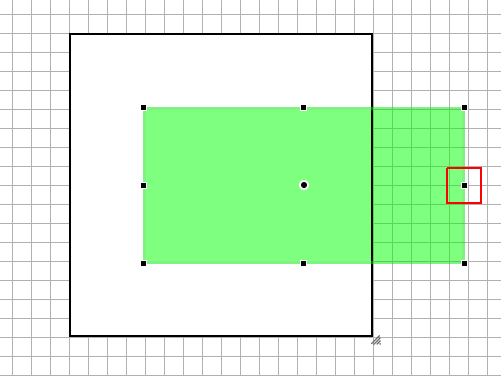
\includegraphics[width=0.5\textwidth]{images/rectangle_grow_left.png}
  \caption{Resizing a part}
  \label{fig:rectangle_grow_left}
\end{figure}

The four squares over the part's \emph{corners}, when clicked and
dragged, will grow or shrink that part on two axes -- those
perpendicular to the two edges touching the respective square. The
other two edges will remain on their initial positions. For example,
in figure \ref{fig:rectangle_grow_diagonal}, the square marked in red
has been dragged rightwards and upwards its original position. That is
why you see \texttt{Rectangle01} now larger in width and shorter in
height.

\begin{figure}[h!]
  \centering
  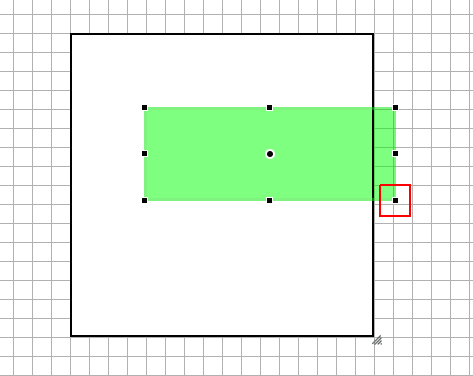
\includegraphics[width=0.5\textwidth]{images/rectangle_grow_diagonal.png}
  \caption{Resizing a part}
  \label{fig:rectangle_grow_diagonal}
\end{figure}

Finally, there's a black \emph{circle} centered over the new part's
visual representation. This is where the user is going to click and
drag in order to \emph{move} the part around, relative to its
group. For example, in figure \ref{fig:rectangle_move},
\texttt{Rectangle01} has been moved to a different position. As you
see, a part may be placed outside the boundaries of its group (it may
be invisible at some state, for example).

\begin{figure}[h!]
  \centering
  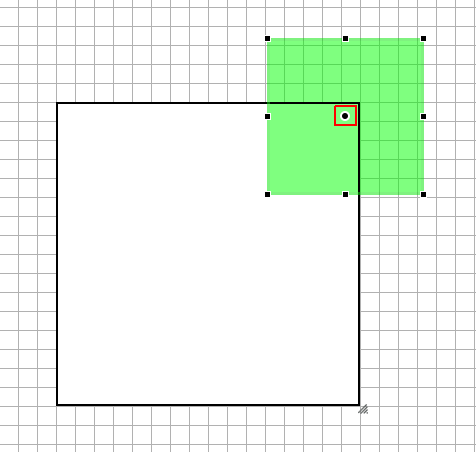
\includegraphics[width=0.5\textwidth]{images/rectangle_move.png}
  \caption{Moving a part}
  \label{fig:rectangle_move}
\end{figure}

All these visual moving and resizing actions will reflect on the
part's property groups on the right of the main window,
naturally. Some of that properties on the collapsables can be changed
directly, what will be seen better further.

Selection of parts happen either when you click over their names on
the parts list or when you click directly over their bodies on the
group displaying area. The second mode of selection is affected by
object stacking, which is addressed on the next section. You'll be
able to select a part in this manner only if the clicked point is not
covered by another part regarding the stacking order. If this is so,
you can always select this specific part by the parts list.

There is a way to unselect all parts, which you achieve by clicking,
on the group displaying area, over a region outside the group
boundaries and with no object underneath.

\subsection{Re-stacking and deleting parts}

To illustrate re-stacking of parts, let's add a new rectangle to our
group, so that it looks really like what was seen in figures
\ref{fig:rectangle_grow_left}, \ref{fig:rectangle_move} and
\ref{fig:rectangle_grow_diagonal}. If you look carefully, there is a
white rectangle as a background on them.

If you click at the \GUIIcon{``+''} icon (region 1 of figure
\ref{fig:new_rectangle}) and add another rectangle, you'll end up with
a part looking exactly as \texttt{Rectangle01}, placed on top of
it. If you accepted the suggested name, while adding it, it will be
named ``\texttt{Rectangle02}''. Let's resize it by directly editing
its size/positioning property values. Figure
\ref{fig:restack_pre_pre}, region 2, highlights the text entries
you'll have to edit and hit the return key to resize
\texttt{Rectangle02}: the \GUIEditable{``relative''} and
\GUIEditable{``offset''} ones. There are two pairs of them, placed
inside the property subgroups named \GUILabel{``top-left''} and
\GUILabel{``bottom-right''}. Make sure \texttt{Rectangle02} is the
selected part and change that values to exactly what is seen on figure
\ref{fig:restack_pre_pre}; the part will be then resized to the
group's dimensions, centered to it, as seen there. You should not care
if it's not clear how this editing had that effect, because it will be
better explained at section \ref{sec:part_states}.

%FIXME: look at the alignment bug after text entry changes
\begin{figure}[h!]
  \centering
  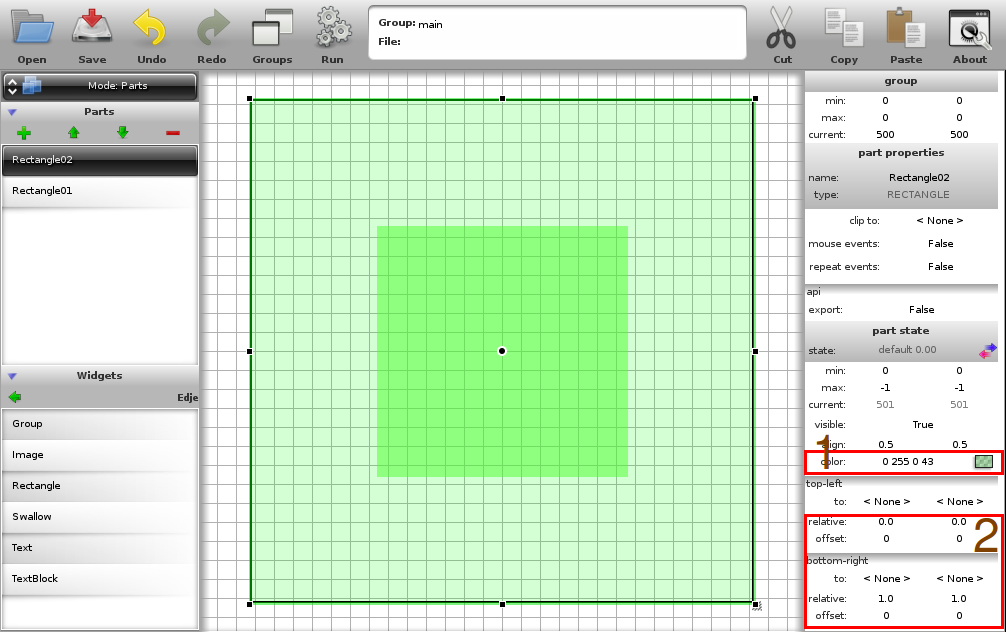
\includegraphics[width=0.95\textwidth]{images/part_resize_entries.png}
  \caption{New rectangle, with size changed}
  \label{fig:restack_pre_pre}
\end{figure}

We now just have to make this new rectangle to look (solid) white.
Look at region 1 of figure \ref{fig:restack_pre_pre}. It highlights
the \GUIEditable{``color''} property of a part (in a given state). It
contains a four integer numbers text entry and a little rectangular
box, which itself is colored with the same color the selected object
has.

Those 4 numbers represent the component values of the part's color (in
RGB space), being them, respectively:

\begin{itemize}
\item red channel
\item green channel
\item blue channel
\item alpha channel
\end{itemize}

One way of altering that color is by directly editing the text entry
and hitting the return key. Another easier way is by clicking over
that colored box on the right. A floating box will appear, just as
depicted in figure \ref{fig:color_box}.

\begin{figure}[h!]
  \centering
  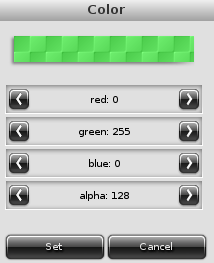
\includegraphics[width=0.3\textwidth]{images/color_box.png}
  \caption{Color selection box}
  \label{fig:color_box}
\end{figure}

To change those four values, just click over the labels \emph{between}
the \GUIButton{``<''} and \GUIButton{``>''} buttons and drag. This
will increase or decrease the respective channel rapidly. Clicking
directly over those same buttons will increase or decrease those
values by one unit, only. A snapshot of the color formed by the
numeric color components is shown in a rectangle on the top of the
color box. By clicking the \GUIButton{``Set''} button, you'll have the
color changed, actually. For our objectives, make those values be
all \emph{255}. After you set the new color, you'll end up with what
is depicted in figure \ref{fig:restack_pre}.

\begin{figure}[h!]
  \centering
  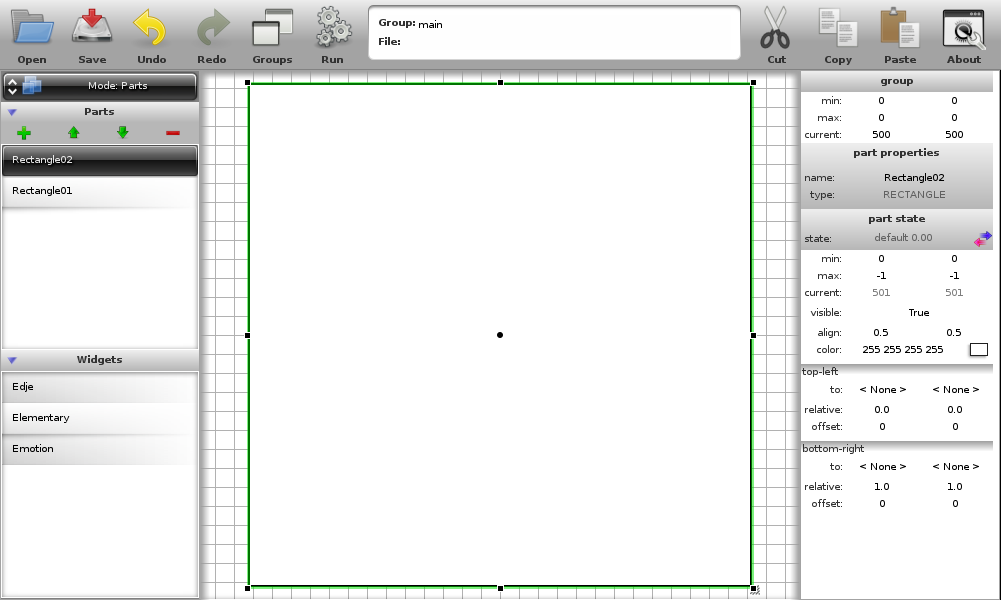
\includegraphics[width=0.95\textwidth]{images/rectangle_stack_pre.png}
  \caption{New rectangle, with size and color changed}
  \label{fig:restack_pre}
\end{figure}

Back to re-stacking, region 1 of figure \ref{fig:new_rectangle} will
exhibit three more action buttons over the actual list of parts,
besides the \GUIIcon{``+''} one, if a part is selected, which are:

\begin{description}
\item[\GUIIcon{upwards arrow}] This is the re-stack \emph{above}
  action.
\item[\GUIIcon{downwards arrow}] This is the re-stack \emph{below}
  action. It does the exact opposite of the former action,
  naturally. If you click on it with \texttt{Rectangle02} selected,
  being it on the state shown in figure \ref{fig:restack_pre}, you'll
  get what is depicted on figure \ref{fig:restack}:
  \texttt{Rectangle01} is now \emph{on top} of the other one.
\item[\GUIIcon{``-''}] This is the part removal action. When clicked,
  the selected part will be totally removed from the group under
  edition, along with all its states.
\end{description}

\begin{figure}[h!]
  \centering
  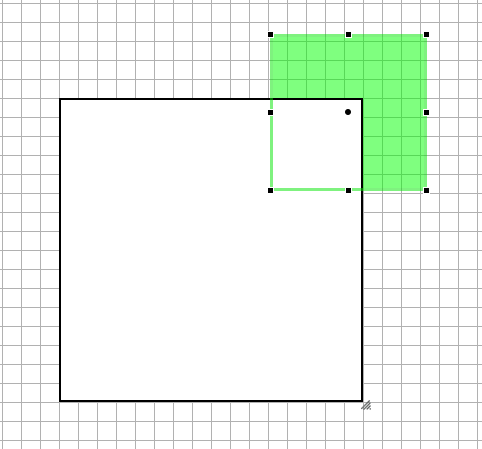
\includegraphics[width=0.95\textwidth]{images/rectangle_stack.png}
  \caption{Re-stacking a part}
  \label{fig:restack}
\end{figure}

\subsection{Part clipping and reaction to mouse events}

Let's start looking better into the properties collapsable groups, on
the right of the main window's screen. The ``part properties'' one,
marked as region 5 in figure \ref{fig:new_rectangle}, has two text
labels which give you the name of the selected part and its type. The
\GUIEditable{``name''} one is actually an \emph{editable} text
entry. By changing its contents and hitting the return key, you'll be
\emph{renaming} the selected part. One will see, additionally, a
\GUILabel{``clip to''} field, which, when clicked, will raise a box
with a list of clipping objects (rectangles) to choose from.

For example, suppose we have, again, those two rectangles --
\texttt{Rectangle01} and \texttt{Rectangle02} -- and a third one,
being it (solid) white, too\footnote{ It's important that it gets the
  color ``\texttt{255 255 255 255}'' (a default clipper
  color).}. Place this third rectangle, which we'll call
\texttt{Rectangle03}, so that it overlaps with \texttt{Rectangle01},
just like in figure \ref{fig:overlap_white}.

\begin{figure}[h!]
  \centering
  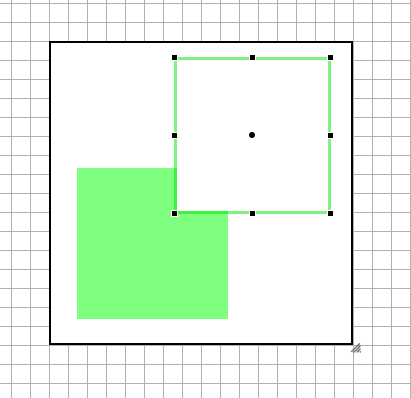
\includegraphics[width=0.5\textwidth]{images/rectangle_overlap_white.png}
  \caption{Overlapping objects}
  \label{fig:overlap_white}
\end{figure}

Back to the \GUILabel{``clip to''} field, you can check that both
rectangles have \GUIEditable{``<None>''} on their entries. This means,
naturally, that they're not clipped to any other part. Select
\texttt{Rectangle01} and click on this field. Another floating box
will appear, just as seen on figure \ref{fig:clipping_box}.

\begin{figure}[h!]
  \centering
  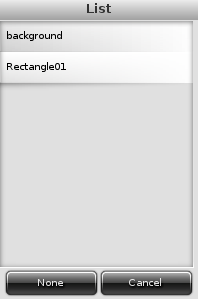
\includegraphics[width=0.3\textwidth]{images/clipping_box.png}
  \caption{Clipper selection box}
  \label{fig:clipping_box}
\end{figure}

All (other) rectangles in the group are candidates to clip the
selected object. We'll choose \texttt{Rectangle03}, here, and the
effect should be something like figure \ref{fig:overlap_clipped}:
\texttt{Rectangle01} has only the area coinciding with
\texttt{Rectangle03} colored green. The rest is shown transparent and
what you see is actually \texttt{Rectangle02}. If you call, to
\texttt{Rectangle01}, the clipper selection box again and click on the
\GUIButton{``None''} button, you'll get again to the state we were in
figure \ref{fig:overlap_white}.

\begin{figure}[h!]
  \centering
  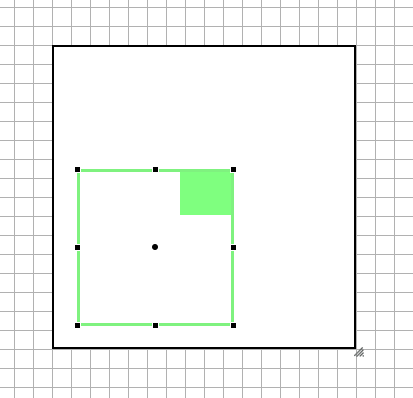
\includegraphics[width=0.5\textwidth]{images/rectangle_overlap_clipping.png}
  \caption{Overlapping objects -- clipper and clippee}
  \label{fig:overlap_clipped}
\end{figure}

To finish the ``part properties'' collapsable group, we have the
\GUIEditable{``mouse events''} and \GUIEditable{``repeat events''}
properties. These are true/false ones which will set the same
properties the underlying evas object has for a given part, i. e.,
whether the object is receiving mouse events and repeating them,
respectively.

\subsection{Part states}
\label{sec:part_states}

Let's now go into the details of the region 7, seen in figure
\ref{fig:new_rectangle}. If we go back to the state we were in that
figure, the cited region looked like figure
\ref{fig:part_state_group}.

\begin{figure}[h!]
  \centering
  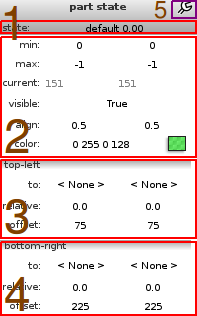
\includegraphics[width=0.3\textwidth]{images/part_state_group.png}
  \caption{The ``part state'' collapsable property group}
  \label{fig:part_state_group}
\end{figure}

This is where the selected part's properties which are \emph{bound to
  a state} are shown and can be edited. The current state under
edition for the part has its name displayed on region 1 (figure
\ref{fig:part_state_group}). Every new part will have only the default
state after creation, which is called ``\texttt{default 0.0}'', as the
reader may know. Except for the default one, states can be renamed by
edition of the \GUIEditable{``name''} entry in this region.

Region 3, in that same figure, has general properties, like
minimum/maximum size hints, visibility flag, alignment inside part's
container and color. All of them are text entries which can be altered
and, after a return key press, have the visual representation updated
on the group displaying area. The \GUILabel{``current''} label you see
is not editable and shows the part's current size based on what is
filled for the two regions below, 4 and 5. These two regions denote,
respectively, the positioning of the \emph{top-left} and
\emph{bottom-right} corners of the the part's container. Figure
\ref{fig:rectangle_rel1rel2} highlights these two points for
\texttt{Rectangle01}, which coincide with two of the part resizing
squares.

\begin{figure}[h!]
  \centering
  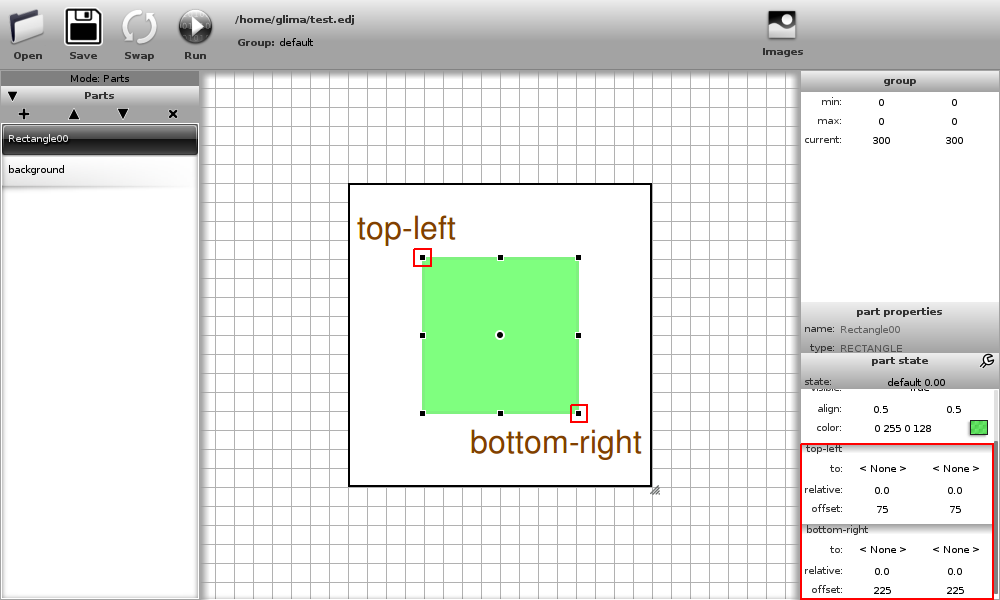
\includegraphics[width=1.0\textwidth]{images/rectangle_rel1rel2.png}
  \caption{A part's top-left and bottom-right anchor points}
  \label{fig:rectangle_rel1rel2}
\end{figure}

Roughly, properties seem inside regions 3, 4 and 5 have the exact
meaning of the homonymous building blocks found in \texttt{.edc}
files.  Their meanings should be straightforward to readers with a
minimal prior knowledge of Edje Data Collections. If you're not
familiar with it, the document ``The Enlightenment Foundation
Libraries -- A Big Picture'' gives a good introduction on them. For
the ones willing to skip it, we quote that text's part on object
relative positioning on appendix \ref{app:edje_pos}.

Figures \ref{fig:visibility_false} to \ref{fig:rel_drag} illustrate
some effects one gets by modifying some of the properties seem on
figure \ref{fig:part_state_group}.

\begin{figure}[h!]
  \centering
  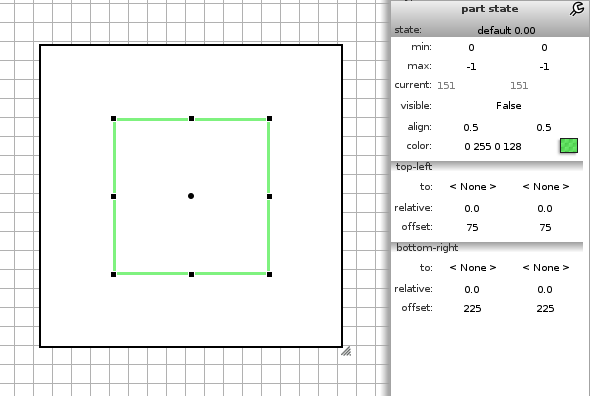
\includegraphics[width=0.88\textwidth]{images/visibility_false.png}
  \caption{Making \texttt{Rectangle01} invisible for state
    \texttt{default 0.0}}
  \label{fig:visibility_false}
\end{figure}

\begin{figure}[h!]
  \centering
  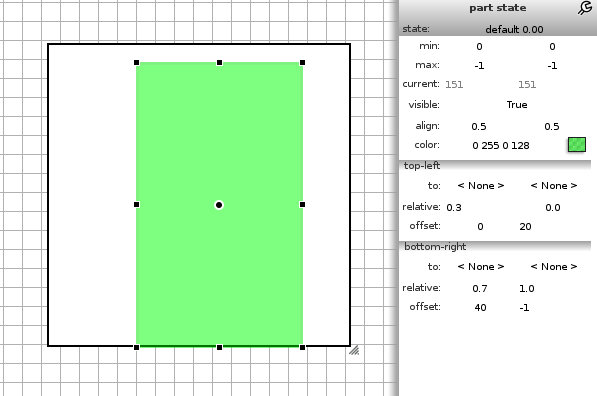
\includegraphics[width=0.88\textwidth]{images/rel_and_offset_changes.png}
  \caption{Changing \texttt{Rectangle01}'s positioning relative to its
    group}
  \label{fig:rel_and_offset_changes}
\end{figure}

\begin{figure}[h!]
  \centering
  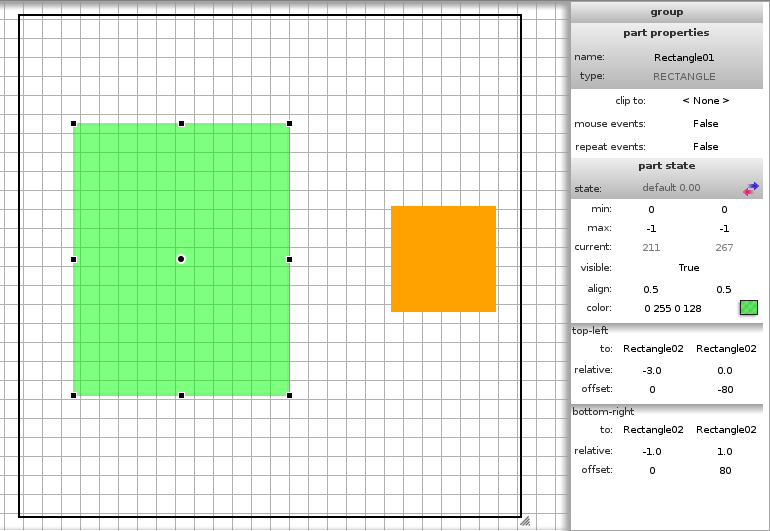
\includegraphics[width=0.88\textwidth]{images/relative_to_other_part.png}
  \caption{Now making \texttt{Rectangle01} relative to another one,
    \texttt{Rectangle02}, whose position can be seen on the group
    displaying area.}
  \label{fig:relative_to_other_part}
\end{figure}

\begin{figure}[h!]
  \centering
  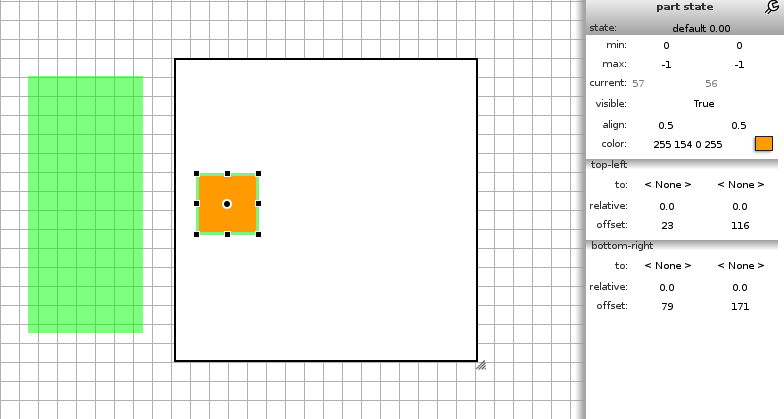
\includegraphics[width=0.88\textwidth]{images/rel_drag.png}
  \caption{This is what one gets by just grabbing \texttt{Rectangle02}
    from the position it had in figure
    \ref{fig:relative_to_other_part} to the one shown here. Because
    \texttt{Rectangle01} is positioned relatively to it, it is also
    moved leftwards, proportionally.}
  \label{fig:rel_drag}
\end{figure}

\subsection{Managing Parts' States}
%TODO: being worked on, let it outdated, for now.

The ``part state'' collapsable group, seen in figure
\ref{fig:part_state_group}, has a region which wasn't cited yet: 2. If
you click on that icon, you'll get the dialog box shown in figure
\ref{fig:states_dialog}.

\begin{figure}[h!]
  \centering
  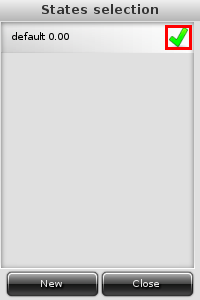
\includegraphics[width=0.28\textwidth]{images/states_box.png}
  \caption{Part states management dialog box}
  \label{fig:states_dialog}
\end{figure}

Before returning to the actions there available, we'll create a
\emph{new state} to \texttt{Rectangle01}, being the default one the
one we get just after adding it to the group.

%FIXME: text entry renames the state, now
Region 1 of figure \ref{fig:part_state_group}, besides showing the
current state's name for a part, is a text entry used to \emph{create}
new states. If you click on it, edit the text changing
\GUIEditable{``default''} to, say, \GUIEditable{``newstate''}, you'll
have just \emph{cloned} the former into the latter. Click again over
the icon in region 5 and you'll see what is depicted on figure
\ref{fig:states_dialog_newstate}.

\begin{figure}[h!]
  \centering
  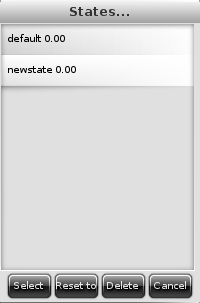
\includegraphics[width=0.28\textwidth]{images/states_box_newstate.png}
  \caption{Note the recently added state, ``newstate''}
  \label{fig:states_dialog_newstate}
\end{figure}

You may, now, change the state dependent properties of the selected
part as you wish. For switching between states of a part, use the
\GUIButton{``Select''} button seen on figure
\ref{fig:states_dialog}. The \GUIButton{``Reset to''} button, on the
same figure, will set the properties seen on the current state to
those of the state selected on the list of that dialog. The
\GUIButton{``Delete''} one will, naturally, delete the current state
and \GUIButton{``Cancel''} will close that dialog.

\section{Types of Parts and their Particularities}

So far, we have only dealt with rectangle parts on the explanation of
Editje's features. The properties of that type of object have been all
described, then. Other types of parts have extra ones (which reflect
on extra GUI entries in Editje), though, which haven't been discussed
yet.

\subsection{Text and Textblock Parts}

If, when on the ``New Part'' dialog, you choose the text type, you'll
end up with a new object which looks like the one shown in figure
\ref{fig:new_text}.

\begin{figure}[h!]
  \centering
  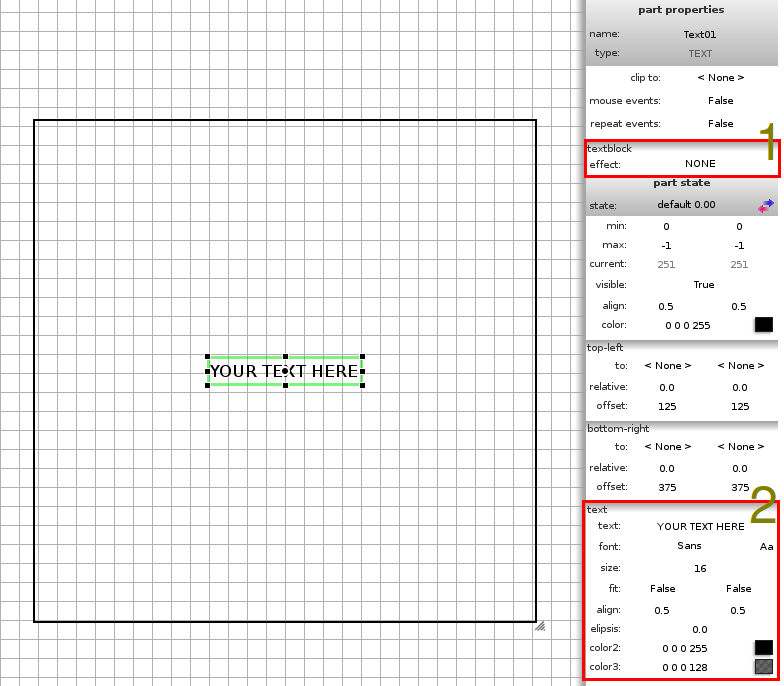
\includegraphics[width=1.0\textwidth]{images/new_text.png}
  \caption{A new text part just created}
  \label{fig:new_text}
\end{figure}

The default text for this text entry part is ``YOUR TEXT HERE'', as
shown there. We also see that text parts have a singular property,
visible under the \GUILabel{``textblock''} tab, inside the ``part
properties'' collapsable group (see region 1, in figure
\ref{fig:new_text}).  This is the \GUIEditable{``effect''} property,
and it does just what you might imagine -- change the effect used
while rendering the part's text. For example, look at what one gets
choosing the ``OUTLINE SOFT SHADOW'' effect, in figure
\ref{fig:text_effect}.

\begin{figure}[h!]
  \centering
  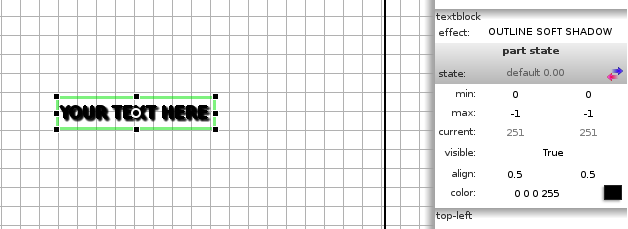
\includegraphics[width=0.8\textwidth]{images/text_effect.png}
  \caption{Text part with effect}
  \label{fig:text_effect}
\end{figure}

In the state dependent properties, we get a new tab of properties for
text parts, called \GUILabel{``text''} (region 2 in figure
\ref{fig:new_text}).  They affect the text part as follows:

\begin{description}
\item[\GUIEditable{``text''}:] The actual text to display.
\item[\GUIEditable{``font''}:] The font to render the text from.
\item[\GUIEditable{``size''}:] The text size.
\item[\GUIEditable{``fit''}:] When any of these entries is set to
  ``True'', Editje will resize the text, so that it to fits in it's
  container, in the respective axis (the \GUIEditable{``size''} is
  ignored, if this property is enabled). Both are disabled by default.
\item[\GUIEditable{``align''}:] Changes the alignment of the actual
  text inside the part's container, ranging from 0 (left) to 1
  (right).
\item[\GUIEditable{``elipsis''}:] Specifies a point along the actual
  text string to be the least probable of being cut out in case of a
  resizing resulting in something smaller than the text itself. Values
  range from 0 to 1, meaning left to right.
\item[\GUIEditable{``color2''}:] Color used as \emph{shadow}, if
  applicable, for the text string.
\item[\GUIEditable{``color3''}:] Color used as \emph{outline}, if
  applicable, for the text string.
\end{description}

We won't exhibit all of the effects above, for brevity, but some of
them are display in figure \ref{fig:text_misc}.

%TODO: check it!
Textblock parts support inside Editje is still being worked on. It
should be completed soon.

%TODO: introduce the fonts wizard, when it's bug free

\begin{figure}[h!]
  \centering
  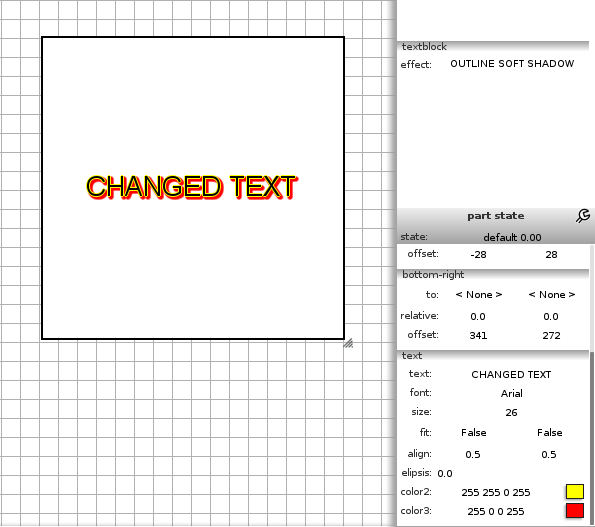
\includegraphics[width=0.9\textwidth]{images/text_misc.png}
  \caption{Text part with ``OUTLINE SOFT SHADOW'' effect, customized
    text string (``CHANGED TEXT''), font (Arial) and size (26) and,
    finally, customized ``color2'' and ``color3'' colors.}
  \label{fig:text_misc}
\end{figure}

\subsection{Image and Gradient Parts}

If the user inserts a new part of the image type, he or she will end
up with something like what is seen in figure \ref{fig:new_image}.
The actual figure part is what is indicated in region 1. It may look
like a transparent rectangle, but it just indicates that you have no
image file set to it yet. What we get specifically for this part type
is the \GUILabel{``image''} tab, indicated in region 2.

\begin{figure}[h!]
  \centering
  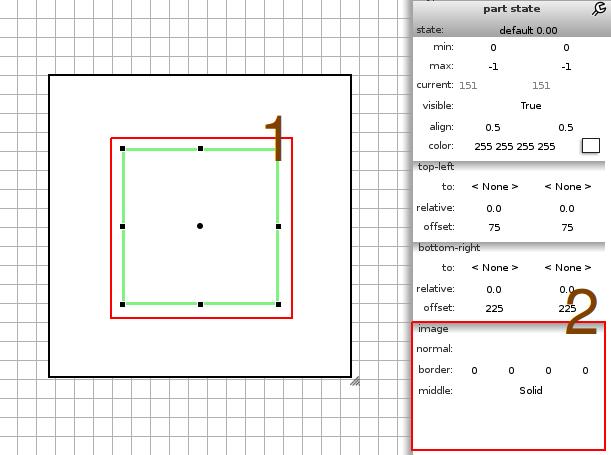
\includegraphics[width=0.9\textwidth]{images/new_image.png}
  \caption{A new image part just created}
  \label{fig:new_image}
\end{figure}

The \GUIEditable{``normal''} property receives a reference to an image
already inserted in the group. Clicking on that box will raise a
dialog very similar to the one seen in figure
\ref{fig:select_an_image}, shown here in figure
\ref{fig:select_an_image_to_part}.

% TODO: re-use it somehow when describing the new dialog form, *when it's
% complete

% presents an icon that will lead the
% user to an \emph{image management} context: it will open a box
% listing all the images used in the current group. By selecting an
% image entry on the list on the left, you get a thumbnail preview of
% it on the right (see figure \ref{fig:select_an_image}). If you click
% on the \GUIButton{``Add new''} button, a file navigation list takes
% the place of the previous one. Whenever you select, on the new list,
% a file of an image, its thumbnail preview will be shown as well (see
% figure \ref{fig:select_an_image_fs}). Click on the
% \GUIButton{``Ok''} button, below the file navigation list, and this
% file will now integrate the list of images of the group (it will be
% possible to set that image to any image part). If you wish to return
% to the images on the group list, just hit
% \GUIButton{``Cancel''}. \GUIButton{``Close''}, naturally, is the
% button which closes the image management dialog entirely.  Editje's
% main screen for other modes of operation will appear in their
% specific sessions.

% \begin{figure}[h!]
%   \centering
%   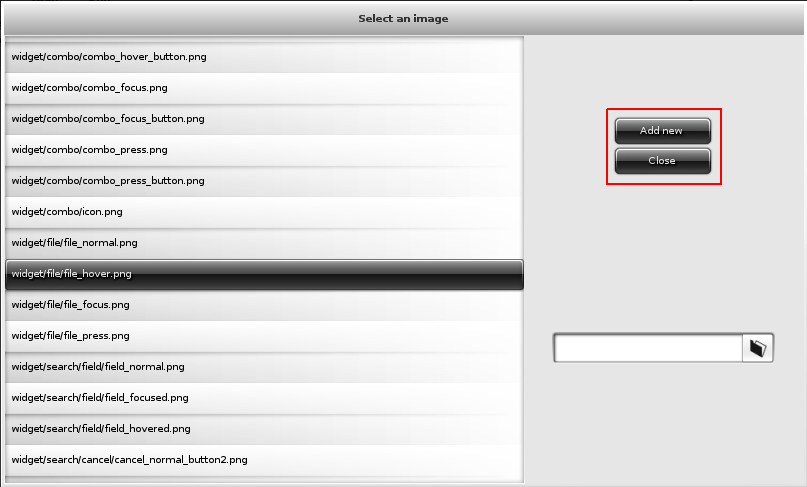
\includegraphics[width=1.0\textwidth]{images/select_an_image.png}
%   \caption{Image management dialog box}
%   \label{fig:select_an_image}
% \end{figure}

% \begin{figure}[h!]
%   \centering
%   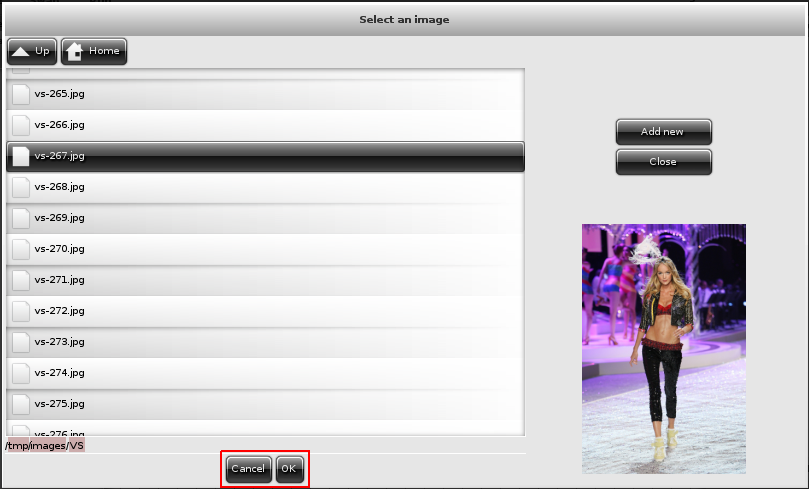
\includegraphics[width=1.0\textwidth]{images/select_an_image_fs.png}
%   \caption{Image management dialog box: adding a new image to the
%     group}
%   \label{fig:select_an_image_fs}
% \end{figure}

% \begin{figure}[h!]
%   \centering
%   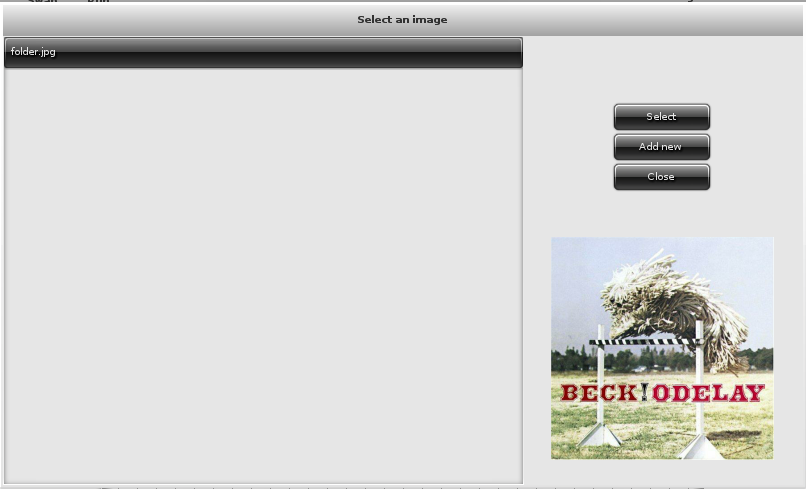
\includegraphics[width=0.95\textwidth]{images/select_an_image_to_part.png}
%   \caption{Image management dialog box: selecting images to image parts}
%   \label{fig:select_an_image_to_part}
% \end{figure}

% Note that, in this new ``Select an image'' dialog, there's an
% exclusive button: \GUIButton{``Select''}. Clicking on it will bind
% that image to the part under selection, what we show in figure
% \ref{fig:image_part}.

% \begin{figure}[h!]
%   \centering
%   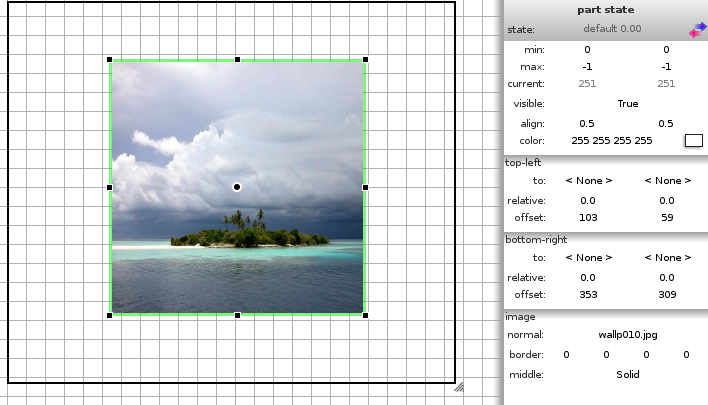
\includegraphics[width=0.95\textwidth]{images/image_part.png}
%   \caption{Image part, now bound to image file}
%   \label{fig:image_part}
% \end{figure}

% TODO: describe them! but when the upper TODO is gone
We won't describe the other two properties in the new tab, for
brevity. Gradient support, inside Editje, is also not completely
finished. It should be ready for use soon.

\subsection{Swallow and Group Parts}

Swallow parts are, roughly speaking, ``holes'' in the current group
into which other edje objects (other groups) can be inserted (or
``swallowed'') \emph{at run time}. Inside Editje, their management is
practically the same as of rectangle parts.

% TODO: finish, then!
Group parts support by Editje is being finished, yet.

\subsection{External Widgets: Elementary}
%FIXME: explain briefly what each kind of widget is/does!

By now, Elementary is the only external module whose widgets have been
made available to edje-edition as common part objects. Region 6 of
figure \ref{fig:new_rectangle}, the list of available widgets/parts,
is a quick way of adding these widgets into the group. The ``Edje''
entry of that list will lead to a list of the ``common'' UI elements
one gets -- the ones implemented directly on the evas or edje
libraries. The ``Elementary'' one, naturally, will list (some) widgets
provided by that library (see figure \ref{fig:elm_widgets}). Each list
entry has an icon illustrating the respective widget. Clicking over
one of them will add that kind of object to the group under edition.

\begin{figure}[h!]
  \centering
  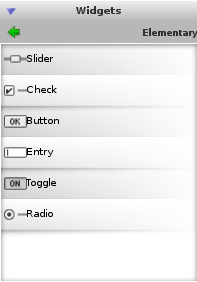
\includegraphics[width=0.3\textwidth]{images/elm_widgets.png}
  \caption{List of Elementary widgets to choose from}
  \label{fig:elm_widgets}
\end{figure}

In what follows, we document the specific properties one finds for
each of those widget parts. All of them have, as extra tabs in the
property collapsable groups, one (and only one) common tab, which is
named \GUILabel{``external''}.

\subsubsection{Button}

We show in figure \ref{fig:new_button} a recently created button part.
The part's specific properties are highlighted on the figure, being
them:

\begin{description}
  \item[\GUIEditable{``label''}:] This is the button label,
    naturally. The default text string for it would be ``label goes
    here'', but in figure \ref{fig:new_button} it has been customized
    to ``CLOSE''.
  \item[\GUIEditable{``icon'':}] This is the icon object to be
    displayed over the button. Elementary's standard set of icons is
    supported and using them is accomplished by entering their name
    strings in this entry. In figure \ref{fig:new_button}, we have
    used the ``close'' one, which is that ``X''-like image.
    %TODO: group parts supported as icon?
\end{description}

The part's type has also been highlighted: note that all external
module ones will share a common type: ``external''.

\begin{figure}[h!]
  \centering
  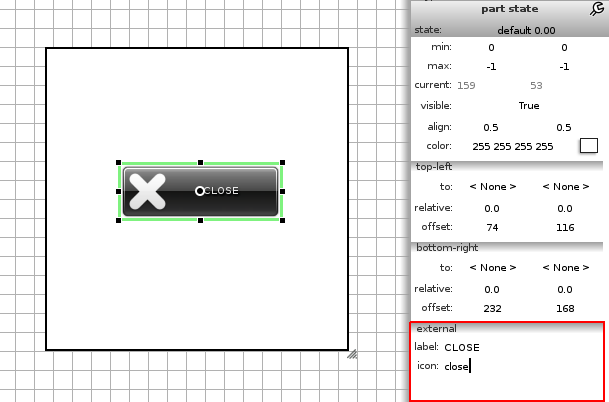
\includegraphics[width=0.9\textwidth]{images/new_button.png}
  \caption{A new button part}
  \label{fig:new_button}
\end{figure}

\subsubsection{Check Box}

Figure \ref{fig:new_checkbox} shows a recently created check box
part. The part's specific properties are highlighted on the figure,
being them:

\begin{description}
  \item[\GUIEditable{``label''}:] Has the same meaning seen on the
    button widget part, and in figure \ref{fig:new_checkbox} it has
    been customized to ``CHECK''.
  \item[\GUIEditable{``icon''}:] Has also the meaning you are familiar
    with. In figure \ref{fig:new_checkbox}, we have used the ``file''
    one.
    %TODO: group parts supported as icon?
  \item[\GUIEditable{``state''}:] This is a boolean property telling
    whether the checkbox should be at checked or unchecked
    state. Clicking on it would draw or erase the tip mark inside the
    box marked in red in \ref{fig:new_checkbox}, besides the ``file''
    icon.
\end{description}

\begin{figure}[h!]
  \centering
  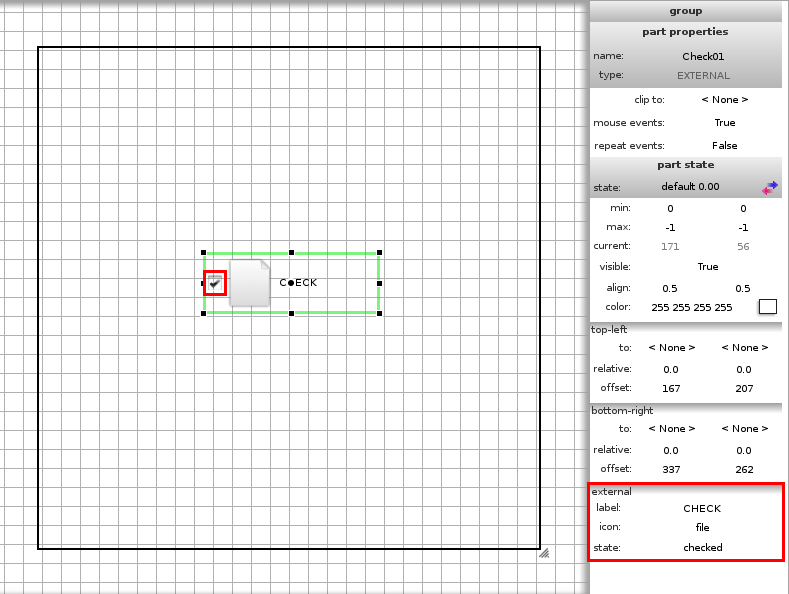
\includegraphics[width=0.89\textwidth]{images/new_checkbox.png}
  \caption{A new check box part}
  \label{fig:new_checkbox}
\end{figure}

\subsubsection{Radio Buttons}

Radio buttons are widgets which make no sense to exist alone: they
appear in \emph{groupings} of two or more. The right way to use them
in Editje is to add as many of these widgets as needed to your group,
assign a value to each one and, then, \emph{group} them together.

Figure \ref{fig:new_checkbox} shows two recently created radio button
parts. Those parts' specific properties are highlighted on the figure,
being them:

%FIXME: these last properties are damn complicated for the end-user
%i won't mind fixing it here too, for a while
\begin{description}
  \item[\GUIEditable{``label''}:] Has the same meaning seen on the
    button widget part.
  \item[\GUIEditable{``icon''}:] Has the same meaning as before.
  \item[\GUIEditable{``group''}:] To define a radio button grouping,
    the user must choose one of the radio button parts in question as
    the \emph{primary one} and, then, set the \GUIEditable{``group''}
    property for all the others to \emph{that part's name}. This
    property, on the primary one, must be left unset.
  \item[\GUIEditable{``value''}:] This is the string to be retrieved
    by the application's back-end, for each of the radio button parts.
\end{description}

\begin{figure}[h!]
  \centering
  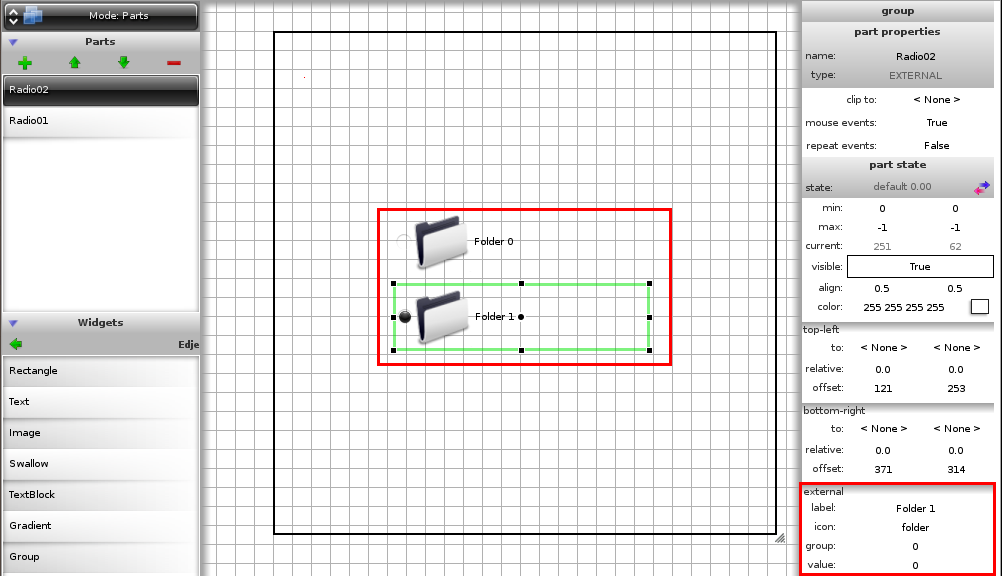
\includegraphics[width=0.9\textwidth]{images/new_radio.png}
  \caption{New radio button parts}
  \label{fig:new_radio}
\end{figure}

\subsubsection{Text Entry}
%FIXME: "text:" property was killed from editje. not updating 'till it gets
%fixed

Figure \ref{fig:new_entry} shows a recently created text entry
part. The part's specific properties are highlighted on the figure,
being them:

\begin{description}
  \item[\GUIEditable{``text''}:] The initial text string to be
    exhibited in the widget.
  \item[\GUIEditable{``single line''}:] Tells whether the text entry
    is single or multi-lined (will enter a line after one presses the
    return key).
  \item[\GUIEditable{``password''}:] This is a boolean property
    telling whether the text entry must or mustn't be in ``password
    mode'', in which it echoes all the characters entered as the ``*''
    one. In figure \ref{fig:new_entry} we have two of these widget
    parts, being one of them in password mode.
\end{description}

\begin{figure}[h!]
  \centering
  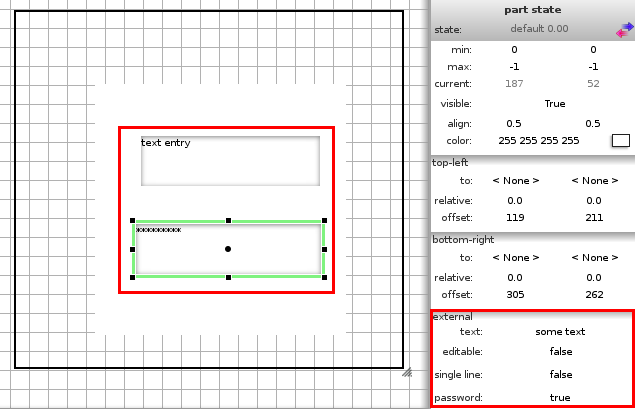
\includegraphics[width=0.87\textwidth]{images/new_entry.png}
  \caption{New text entry parts}
  \label{fig:new_entry}
\end{figure}

\subsubsection{Slider}

We have an example of a recently created slider part in figure
\ref{fig:new_slider}. Its specific properties are highlighted on the
figure, being them:

\begin{description}
  \item[\GUIEditable{``label''}:] Text label for the widget.
  \item[\GUIEditable{``icon''}:] Icon decorating it, if set.
  \item[\GUIEditable{``min''}:] Minimum value it can be set to.
  \item[\GUIEditable{``max''}:] Maximum value it can be set to.
  \item[\GUIEditable{``value''}:] Current displaying value.
  \item[\GUIEditable{``horizontal''}:] Whether the slider has
    horizontal or vertical sliding direction.
  \item[\GUIEditable{``inverted''}:] Whether the slider grows from
    beginning to end or the contrary. That translates to from top to
    bottom and from left to right, for vertical and horizontal
    aspects, respectively.
  \item[\GUIEditable{``span''}:] This sets the minimum width or height
    (depending on orientation) of the knob the GUI user will actually
    drag.
  \item[\GUIEditable{``unit format''}:] Sets the format of the string
    displaying the slider's value, besides it.
  \item[\GUIEditable{``indicator format''}:] Sets the format of the
    string displaying the slider's value \emph{while it's being
      dragged}, on top of the knob.
\end{description}

\begin{figure}[h!]
  \centering
  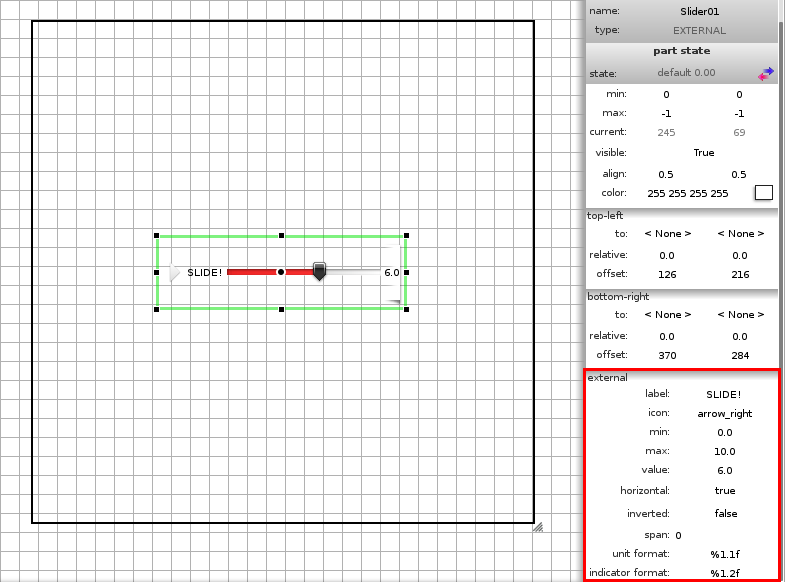
\includegraphics[width=0.9\textwidth]{images/new_slider.png}
  \caption{New slider part}
  \label{fig:new_slider}
\end{figure}

\subsubsection{Toggle}

An Elementary toggle is a widget which records a boolean value, fed by the
GUI user. An example of a recently created toggle part can be seen in figure
\ref{fig:new_toggle}. Its specific properties are highlighted on the
figure, being them:

\begin{description}
  \item[\GUIEditable{``label''}:] Text label for the widget.
  \item[\GUIEditable{``icon''}:] Icon decorating it, if set.
  \item[\GUIEditable{``label on''}:] The label for its knob, at the
    ``on'' (true) state.
  \item[\GUIEditable{``label off''}:] The label for its knob, at the
    ``off'' (false) state.
  \item[\GUIEditable{``state''}:] Current state of the widget.
\end{description}

\begin{figure}[h!]
  \centering
  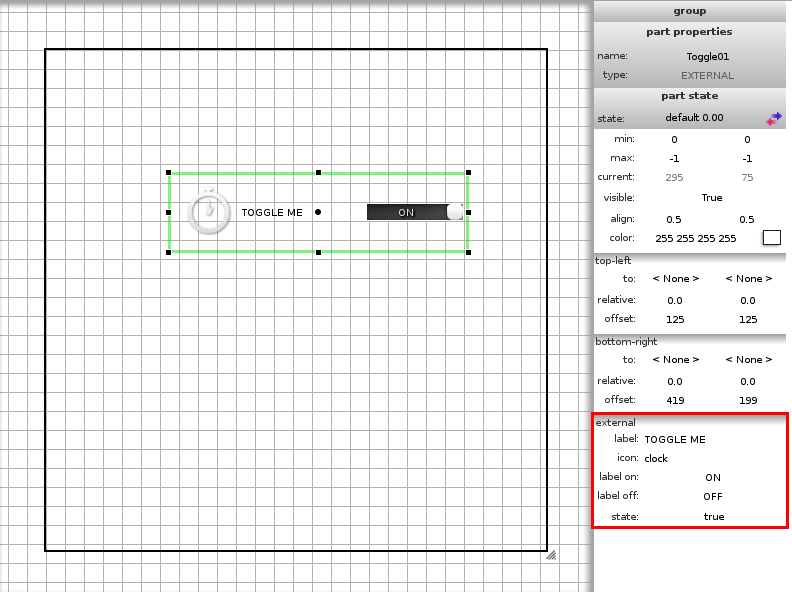
\includegraphics[width=0.9\textwidth]{images/new_toggle.png}
  \caption{New toggle part}
  \label{fig:new_toggle}
\end{figure}

%FIXME: document the "group" collapsable
% The ``group'' one will list the group's properties, naturally, which
% at the time are:
%   \begin{itemize}
%     \item group's minimum and maximum size hints
%     \item group's default (current) size.
%   \end{itemize}

\section{Animations}
\label{animation_editing}

Animations are programs ran one after another, setting the
corresponding state to the affected parts. This is handled within
Editje using special names to hide this programs and states from the
user and avoid tampering with them in other editing modes. This should
not normally be a problem, but it's worth noting in the case where
\texttt{.edc} files are edited, as opening the file in a standard text
editor \emph{won't} do anything to protect the animations from being
wrongly altered.

Once in Animation mode, you will find yourself in front of the window
shown in figure \ref{fig:animation_mode_numbers}.

\begin{figure}[h!]
  \centering
  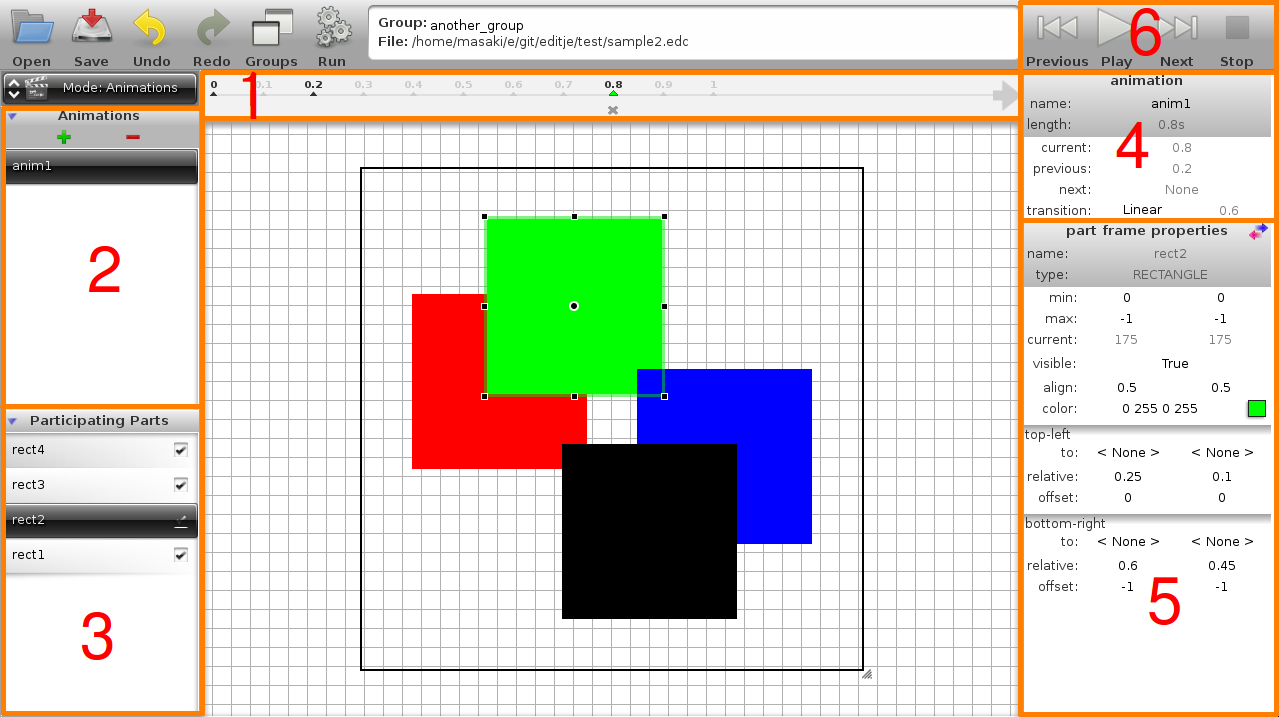
\includegraphics[width=1.0\textwidth]{images/animation_mode_numbers.png}
  \caption{The animation mode}
  \label{fig:animation_mode_numbers}
\end{figure}

\begin{description}
\item[1 -- Timeline] Here are shown the frames the currently selected
  animation is composed of. Each mark in it is a \emph{point in time},
  not a frame number. What this means is, to add frames to an
  animation, you select the time you want that frame to be, 0 being
  always there as it is the initial state of the animation, 0.1 being
  the animation at 0.1 seconds, and so on.  This will be further
  explained later on in this document.
\item[2 -- Animations list] The list of available animations in the
  group being edited. Selecting one will update the timeline
  accordingly and set all parts to the initial state.
\item[3 -- Parts list] The list of all parts in the group, but unlike
  the ``Parts'' mode, this only lets you select a part. It's not
  possible in this mode to add or remove parts, nor to change their
  stacking order.
\item[4 -- Frame details] Shows the previous, current and next
  \emph{times} for the currently selected frame, as well as the
  transition style and duration. The transition style operates over
  the duration of the frame and not on its movement. This will be
  explained in more detail later.
\item[5 -- Part state details] Properties of the currently selected
  part, in the current frame. Just like in ``Parts'' mode, but it's
  not possible to change state. However, you can use other states as
  templates and just copy them over by clicking on the little
  \GUIIcon{wrench icon}.
\item[6 -- Animation controls] \GUIIcon{``Previous''} and
  \GUIIcon{``Next''} will jump to the respective \emph{existing}
  frame. \GUIIcon{``Play''} plays the animation in the editor window
  and \GUIIcon{``Stop''} will cancel the animation if playing.
\end{description}

Looking closer to the timeline we see that some times are black and
some are grayed out. The black ones are existing frames in the
animation and we can jump to these states by clicking on them. By
clicking on a grey dot, a new frame is added, creating the necessary
states by copying them from the previous frame in the timeline. In the
future, this new states could be generated by interpolating from the
previous and following frame to form an intermediate state, making it
easier to create fluent animations.

\begin{figure}[h!]
  \centering
  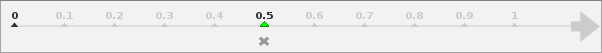
\includegraphics{images/animation_timeline.png}
  \caption{The timeline}
  \label{fig:animation_timeline}
\end{figure}

The marker below the dots indicates the frame being currently edited.

On the animations list we can also see three icons. Marked on figure
\ref{fig:animation_list}, this icons are:
\begin{itemize}
\item 1. \GUIIcon{Hide list}: Hides the list, making more room for the
  Parts list
\item 2. \GUIIcon{New animation}: Pops up the ``New Animation'' dialog
\item 3. \GUIIcon{Delete animation}: Deletes the current animation
\end{itemize}

\begin{figure}[h!]
  \centering
  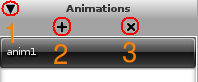
\includegraphics{images/animation_list.png}
  \caption{List of available animations}
  \label{fig:animation_list}
\end{figure}

Be warned that there is no confirmation on deletion yet, so clicking
on delete will effectively remove the animation with no way to bring
it back.

Clicking on \GUIIcon{``New Animation''} will show the dialog in figure
\ref{fig:animation_dialog_new}. In this dialog, just type the name of
the new animation and click \GUIButton{``Add''} or press the return
key to create the animation. If one with the same name already exists,
you will be prompted to choose another one.

\begin{figure}[h!]
  \centering
  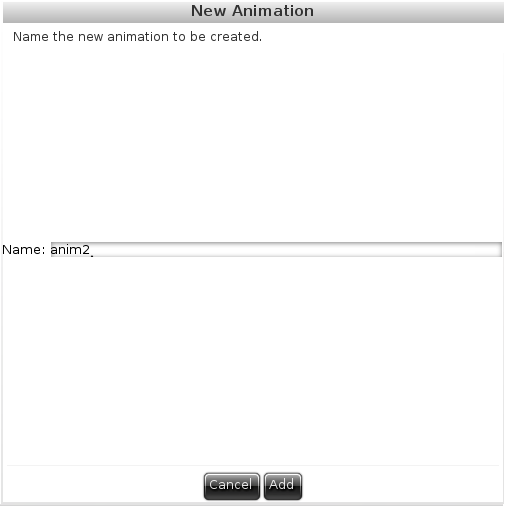
\includegraphics{images/animation_dialog_new.png}
  \caption{New animation dialog}
  \label{fig:animation_dialog_new}
\end{figure}

Adding a new animation will create the initial state based on the
``default'' state of the parts.

For the frame details, as shown on figure
\ref{fig:animation_frame_details}, we can see the timestamps of the
\GUILabel{current}, \GUILabel{previous} and \GUILabel{next} frames,
all of them just for quick access to this information.

\begin{figure}[h!]
  \centering
  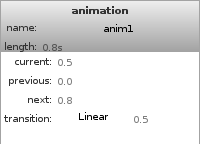
\includegraphics{images/animation_frame_details.png}
  \caption{Details for animation frames}
  \label{fig:animation_frame_details}
\end{figure}

The \GUILabel{``transition''} property lets us change how Edje
interpolates between the two frames. In the future, it will also be
able to change the duration of this transition, which would also alter
the timeline and timestamps of the frames.

An important thing to be noted is that the type of the interpolation
affects the speed of the transition, and not the transition
itself. This means that having a part move from one corner of the
group to the opposite one, and setting the transition to
\emph{SINUSOIDAL} will still make for a linear movement from one state
to the other, but with the speed of this movement changing throughout
its duration.

The transition styles available, are as shown in figure
\ref{fig:animation_transitions}:
\begin{description}
\item[NONE] No interpolation. The part will remain in the state it is
  for the duration of the transition, and when it's done switch to the
  new state instantaneously.
\item[LINEAR] Linear interpolation between the two states. Will move
  from one to the other at a constant speed.
\item[SINUSOIDAL] Speed variations along the transition.
\item[ACCELERATE/DECELERATE] Respectively increase and decrease the
  speed of the state change.
\end{description}

\begin{figure}[h!]
  \centering
  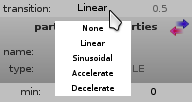
\includegraphics{images/animation_transitions.png}
  \caption{Types of state transition}
  \label{fig:animation_transitions}
\end{figure}

  The part details, as shown in figure \ref{fig:animation_part_details} is
  just like the state details in ``Parts'' mode, with the exception that
  it's not possible to add or delete states, nor switch to another one in
  any other way than changing the animation frame.

\begin{figure}[h!]
  \centering
  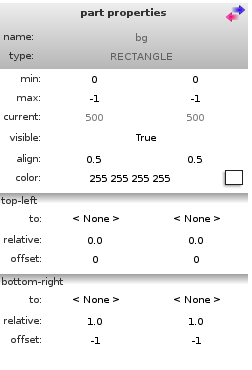
\includegraphics{images/animation_part_details.png}
  \caption{Part details in animation mode}
  \label{fig:animation_part_details}
\end{figure}

  However, it is possible to use states created in the ``Parts'' mode
  as templates by just copying them over the current one. To do this,
  click on the \GUIIcon{wrench icon} marked in figure
  \ref{fig:animation_part_options} to show the ``States'' pop-up as
  depicted in figure \ref{fig:animation_states_popup}, select the
  desired state from the list and click \GUIButton{``Reset to''}. This
  will copy all properties from the state selected to the one being
  edited.

\begin{figure}[h!]
  \centering
  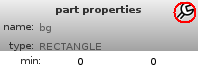
\includegraphics{images/animation_part_options.png}
  \caption{Part options}
  \label{fig:animation_part_options}
\end{figure}

\begin{figure}[h!]
  \centering
  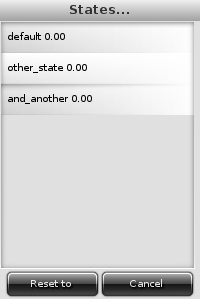
\includegraphics{images/animation_states_popup.png}
  \caption{Copy from state in animations mode}
  \label{fig:animation_states_popup}
\end{figure}

\subsection{A Basic Example}

Now we are going to show the workflow of animation creation and edition
with a couple of simple examples. In order to show them running we will
touch some parts of the Signals mode. For more information on those,
refer to the relevant section in \ref{sec:signal_editing}.

At this point we assume that the user is familiar with part editing, so
this things won't be shown in much detail.

\subsubsection{The Basic Layout}

For this example we will use only Edje, so we are going to stick to simple
parts. We'll start by defining the basic layout of our ``UI'' to have a
couple of ``buttons'' and some sort of indicator of something.

Launch Editje, select \GUIButton{``New''} and pick a name for the
file to start working on an empty group.

Add a Rectangle named ``bg'', make it white and set the relative values to
\begin{verbatim}
top-left:
  to:       < None >   < None >
  relative: 0.0        0.0
  offset:   0          0

bottom-right:
  to:       < None >   < None >
  relative: 1.0        1.0
  offset:   -1         -1
\end{verbatim}

Next, a few more rectangles to represent the buttons and very basic
progress bar.
\begin{description}
\item[``btn.on'']:
\begin{verbatim}
color: 70 200 70 255
top-left:
  to:       bg   bg
  relative: 0.1  0.95
  offset:   0    -25
bottom-right:
  to:       bg   bg
  relative: 0.4  0.95
  offset:   -1   -1
part properties:
  mouse events: True
\end{verbatim}
\item[``btn.off'']:
\begin{verbatim}
color: 200 70 70 255
top-left:
  to:       bg   bg
  relative: 0.6  0.95
  offset:   0    -25
bottom-right:
  to:       bg   bg
  relative: 0.9  0.95
  offset:   -1   -1
part properties:
  mouse events: True
\end{verbatim}
\item[``scr.bg'']:
\begin{verbatim}
color: 0 0 0 255
top-left:
  to:       bg   bg
  relative: 0.0  0.0
  offset:   1    1
bottom-right:
  to:       bg   bg
  relative: 1.0  0.9
  offset:   -2   -25
\end{verbatim}
\item[``scr.border'']:
\begin{verbatim}
color: 240 240 240 255
top-left:
  to:       scr.bg   scr.bg
  relative: 0.0      0.0
  offset:   1        1
bottom-right:
  to:       scr.bg   scr.bg
  relative: 1.0      1.0
  offset:   -2       -2
\end{verbatim}
\item[``scr.content'']:
\begin{verbatim}
color: 0 0 0 255
top-left:
  to:       scr.border   scr.border
  relative: 0.0          0.0
  offset:   2            2
bottom-right:
  to:       scr.border   scr.border
  relative: 1.0          1.0
  offset:   -3           -3
\end{verbatim}
\item[``marker1'']:
\begin{verbatim}
color: 10 10 10 255
top-left:
  to:       scr.content   scr.content
  relative: 0.1           0.7
  offset:   0             0
bottom-right:
  to:       scr.content   scr.content
  relative: 0.3           0.9
  offset:   -1            -1
\end{verbatim}
\item[``marker2'']:
\begin{verbatim}
color: 10 10 10 255
top-left:
  to:       scr.content   scr.content
  relative: 0.4           0.7
  offset:   0             0
bottom-right:
  to:       scr.content   scr.content
  relative: 0.6           0.9
  offset:   -1            -1
\end{verbatim}
\item[``marker3'']:
\begin{verbatim}
color: 10 10 10 255
top-left:
  to:       scr.content   scr.content
  relative: 0.4           0.4
  offset:   0             0
bottom-right:
  to:       scr.content   scr.content
  relative: 0.6           0.6
  offset:   -1            -1
\end{verbatim}
\item[``marker4'']:
\begin{verbatim}
color: 10 10 10 255
top-left:
  to:       scr.content   scr.content
  relative: 0.7           0.7
  offset:   0             0
bottom-right:
  to:       scr.content   scr.content
  relative: 0.9           0.9
  offset:   -1            -1
\end{verbatim}
\item[``marker5'']:
\begin{verbatim}
color: 10 10 10 255
top-left:
  to:       scr.content   scr.content
  relative: 0.7           0.4
  offset:   0             0
bottom-right:
  to:       scr.content   scr.content
  relative: 0.9           0.6
  offset:   -1            -1
\end{verbatim}
\item[``marker6'']:
\begin{verbatim}
color: 10 10 10 255
top-left:
  to:       scr.content   scr.content
  relative: 0.7           0.1
  offset:   0             0
bottom-right:
  to:       scr.content   scr.content
  relative: 0.9           0.3
  offset:   -1            -1
\end{verbatim}
\end{description}

Now some labels for the buttons. For these we'll add two parts of type
``TEXT'' with the following parameters

\begin{description}
\item[``label.on'']:
\begin{verbatim}
color: 0 0 0 255
top-left:
  to:       btn.on   btn.on
  relative: 0.0      0.0
  offset:   0        0
bottom-right:
  to:       btn.on   btn.on
  relative: 1.0      1.0
  offset:   -1       -1
text:
  text: Turn on
  font: Sans:style=Bold
  size: 12
part properties:
  repeat events: True
\end{verbatim}
\item[``label.off'']:
\begin{verbatim}
color: 0 0 0 255
top-left:
  to:       btn.off   btn.off
  relative: 0.0       0.0
  offset:   0         0
bottom-right:
  to:       btn.off   btn.off
  relative: 1.0       1.0
  offset:   -1        -1
text:
  text: Turn off
  font: Sans:style=Bold
  size: 12
part properties:
  repeat events: True
\end{verbatim}
\end{description}

At this point, we should be looking at something like the figure
\ref{fig:anim1_layout}.

\begin{figure}[h!]
  \centering
  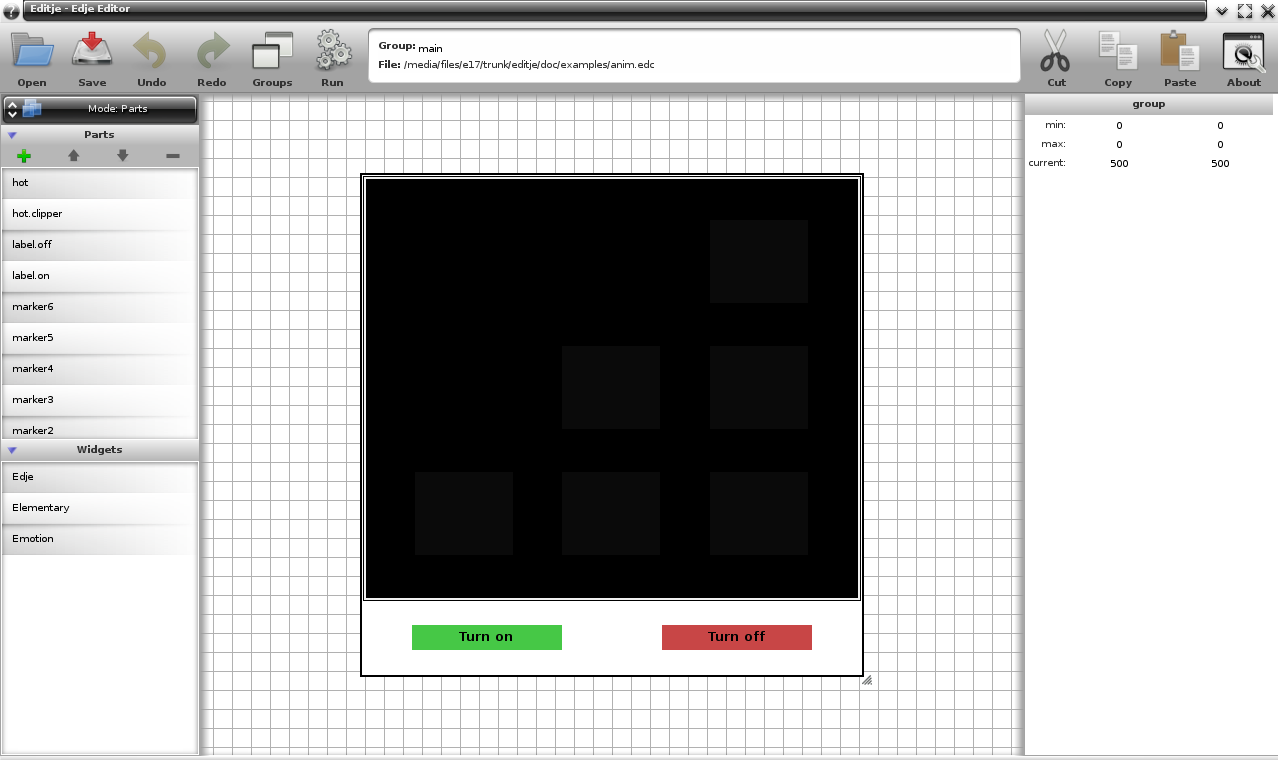
\includegraphics[width=1.0\textwidth]{examples/anim1_layout.png}
  \caption{Example of animations: Setting up the UI}
  \label{fig:anim1_layout}
\end{figure}

And just for fun, I added another text part with a clipper.

\begin{description}
\item[``hot.clipper'']:
\begin{verbatim}
color: 255 255 255 255
top-left:
  to:       scr.content   scr.content
  relative: 0.1           0.3
  offset:   0             0
bottom-right:
  to:       scr.content   scr.content
  relative: 0.6           0.3
  offset:   -1            -1
\end{verbatim}
\item[``hot'']:
\begin{verbatim}
color: 255 0 0 255
top-left:
  to:       scr.content   scr.content
  relative: 0.1           0.1
  offset:   0             0
bottom-right:
  to:       scr.content   scr.content
  relative: 0.6           0.3
  offset:   -1            -1
text:
  text: HOT!
  font: Sans
  size: 16
  fit:  True   False
  color2: 200 0 0 255
  color3: 0 0 0 128
part properties:
  clip to: hot.clipper
  effect: Glow
\end{verbatim}
\end{description}

%  Now we need to create some template states for the parts involved in the
%  animations, to make it easier later. For this, click on the state name
%  for each part, type the ``on'' and press enter.
%
%  For the three markers in the bottom row, we'll set the color to ``0 255
%  0 255'', for the two in the middle ``255 255 0 255'' and for the last
%  one on the top ``255 0 0 255''.
%
%  Next, set ``hot.clipper'' to show the label, changing \emph{top-left}'s
%  \emph{relative} value to be ``0.1  0.1''. For this part, we are also going
%  to need an ``off'' state, with values:
%  \begin{verbatim}
%  top-left:
%    relative: 0.35   0.2
%  bottom-right:
%    relative: 0.35   0.2
%  \end{verbatim}
%
  \subsubsection{The Animations}

Now we are ready to switch to \emph{Animation Mode}. In here, we will
create three animations, which will run one after the other, changing
themselves with \emph{Signals}.

Time for an important note: every animation created in Editje has
three signals associated to it, all of which use the name of the
animation for the ``source'' parameter. This signals are
\begin{itemize}
\item[animation,play]: send it to the Edje object to play the
  animation.
\item[animation,stop]: send it to the Edje object to stop the
  animation.
\item[animation,end]: emitted by the Edje object when the animation
  ends.
\end{itemize}

With all this information, we'll now create the animations. First add
one named ``level1.on''. For this one, we'll start with the default
states for all parts and take it from there to the state seen in
figure \ref{fig:anim1_level1}.

To get there, we'll start by clicking in the timeline, on
\GUIIcon{0.1} to select the first frame, choose the \emph{marker1}
part and set its color to ``0 100 0 255''. Next jump to \GUIIcon{0.2}
and set color to ``0 200 0 255'', then choose \emph{marker2} and set
its color to ``0 100 0 255''. Now go to \GUIIcon{0.3} and set the
color for \emph{marker1} to ``0 255 0 255'', for \emph{marker2} to ``0
200 0 255'' and \emph{marker3} to ``0 100 0 255''.  In \GUIIcon{0.4}
set \emph{marker1} and \emph{marker2} to ``0 255 0 255'', and
\emph{marker3} to ``0 200 0 255''. Finally, in \GUIIcon{0.5}, set the
color for all three of them to ``0 255 0 255''.

\begin{figure}[h!]
  \centering
  \includegraphics[width=1.0\textwidth]{examples/anim1_level1.png}
  \caption{Example of animations: Animating the first level}
  \label{fig:anim1_level1}
\end{figure}

On to the second level. Add another animation, called ``level2.on''
that we will use to animate the middle row of markers. For this
animation, we want to start where the previous one ended, so for the
initial state, set the color of all three markers in the bottom to ``0
255 0 255'' as they were on the last frame of ``level1.on''.

We want this animation to go slower, so pick the first frame in time
\GUIIcon{0.2} and set the color of \emph{marker4} to ``100 100 0 255''.
Now go to \GUIIcon{0.4} and set it to ``200 200 0 255'', and for
\emph{marker5} use ``100 100 0 255''. Then in \GUIIcon{0.6} we'll have
``255 255 0 255'' and ``200 200 0 255'', and in the end both of them
to ``255 255 0 255'' in time \GUIIcon{0.8}.

At this point we should be looking at figure \ref{fig:anim1_level2}.

\begin{figure}[h!]
  \centering
  \includegraphics[width=1.0\textwidth]{examples/anim1_level2.png}
  \caption{Example of animations: Animating the second level}
  \label{fig:anim1_level2}
\end{figure}

Now, for the last animation, create a new one named ``level3.on'', and
make all first 5 markers to look just like they did at the end of
``level2.on''. On this one, we'll also make the label visible by
resizing the clipper along the turning of the last marker.

Click on \GUIIcon{0.4}, choose the part \emph{hot.clipper} and set the
relative value of top-left to ``0.1 0.2''. For \emph{marker6}, set
color to ``100 0 0 255''. Now go to \GUIIcon{0.8} and set the color to
``200 0 0 255'' and relative to ``0.1 0.1''. And with the current
limit, we'll end the animation in \GUIIcon{1.0}, repeating the values
for the \emph{hot.clipper} and setting the color of \emph{marker6} to
``255 0 0 255''.

Figure \ref{fig:anim1_level3} should be the state of the animation by
now.

\begin{figure}[h!]
  \centering
  \includegraphics[width=1.0\textwidth]{examples/anim1_level3.png}
  \caption{Example of animations: Last level animated}
  \label{fig:anim1_level3}
\end{figure}

  \subsubsection{Making the animations runnable}

With the animations over, it's time to connect them to signals so we
can trigger them. Switch to \emph{Signals Mode} and add a new signal
of type \emph{Animation}. Let's call it ``turn.on''. On the right side
of the window are the signal properties. Set \GUIEditable{``signal''}
to ``mouse,clicked,1'' and \GUIEditable{``source''} to ``btn.on'' by
typing these values in there. This will make our signal react to mouse
clicks on the ``Turn on'' button. Then click on the
\GUIEditable{``action''} property to pop up the list of animations and
choose \emph{level1.on}. Now, when clicking on the button, the first
animation will run.

But this is not enough, we want all the animations to run, one after
the other, so we need to somehow hook them together. To do this, add
another signal, this time of type \emph{Signal}, and name it
``turn.on.2''. On the right side there are two instances of
\GUIEditable{``signal''} and \GUIEditable{``source''} now, the ones
above are what the signal listens to in order to be executed, the ones
below are emitted by it, kind of like a proxy. Set the first signal
and source to ``animation,end'' and ``level1.on'', so the signal runs
when the first animation ends, and the other two to ``animation,play''
and ``level2.on''. Now, when the first animation ends, our new signal
will get notified of it and send the play signal to the second
animation.

Add another signal, again of type \emph{Signal}, named ``turn.on.3'',
this time listening to ``animation,end'' from ``level2.on'', and
emitting ``animation,play'' for ``level3.on''. We should have a setup
like seen in figure \ref{fig:anim1_signal_level2}.

\begin{figure}[h!]
  \centering
  \includegraphics[width=1.0\textwidth]{examples/anim1_signal_level2.png}
  \caption{Example of animations: Connecting animations with signals}
  \label{fig:anim1_signal_level2}
\end{figure}

Press the \GUIButton {Run} button in the toolbar and click on the
\emph{Turn on} button to see the animation running.

And to finalize this example, making the \emph{Turn off} button have
the opposite effect should make for a good exercise of everything
we've seen so far.

\section{Signals}
\label{sec:signal_editing}

Signals in Editje is the way of interact easier with the UI using
messages exchange.

\subsection{Evas Callbacks}
All objects in screen with EFL are Evas objects and have callbacks to
listen events. Here we list all callback types of Evas objects:

\begin{description}
\item[EVAS\_CALLBACK\_MOUSE\_IN] This event is triggered when the
  mouse pointer enters the region of the object. This may occur by the
  mouse pointer being moved or by the object being shown, raised,
  moved, resized, or other objects being moved out of the way, hidden,
  lowered or moved out of the way.

\item[EVAS\_CALLBACK\_MOUSE\_OUT] This event is triggered exactly like
  EVAS\_CALLBACK\_MOUSE\_IN is, but occurs when the mouse pointer
  exits an object.  Note that no out events will be reported if the
  mouse pointer is implicitly grabbed to an object (the mouse buttons
  are down at all and any were pressed on that object). An out event
  will be reported as soon as the mouse is no longer grabbed (no mouse
  buttons are depressed). Out events will be reported once all buttons
  are released, if the mouse has left the object.

\item[EVAS\_CALLBACK\_MOUSE\_DOWN] This event is triggered by a mouse
  button being depressed while over an object. If pointer mode is in
  auto-grab mode (default) this causes this object to passively grab
  the mouse until all mouse buttons have been released.  That means if
  this mouse button is the first to be pressed, all future mouse
  events will be reported to only this object until no buttons are
  down. That includes mouse move events, in and out events, and
  further button presses. When all buttons are released, event
  propagation occurs as normal.

\item[EVAS\_CALLBACK\_MOUSE\_UP] This event is triggered by a mouse
  button being released while over an object or when passively grabbed
  to an object. If this is the last mouse button to be raised on an
  object then the passive grab is released and event processing will
  continue as normal.

\item[EVAS\_CALLBACK\_MOUSE\_MOVE]This event is triggered by the mouse
  pointer moving while over an object or passively grabbed to an
  object.

\item[EVAS\_CALLBACK\_MOUSE\_WHEEL] This event is triggered by the
  mouse wheel being rolled while over an object or passively grabbed
  to an object.

\item[EVAS\_CALLBACK\_FREE] This event is triggered just before Evas
  is about to free all memory used by an object and remove all
  references to it. This is useful for programs to use if they
  attached data to an object and want to free it when the object is
  deleted. The object is still valid when this callback is called, but
  after this callback returns, there is no guarantee on the object's
  validity.

\item[EVAS\_CALLBACK\_KEY\_DOWN] This callback is called when a key is
  pressed and the focus is on the object, or a key has been grabbed to
  a particular object which wants to intercept the key press
  regardless of what object has the focus.

\item[EVAS\_CALLBACK\_KEY\_UP] This callback is called when a key is
  released and the focus is on the object, or a key has been grabbed
  to a particular object which wants to intercept the key release
  regardless of what object has the focus.

\item[EVAS\_CALLBACK\_FOCUS\_IN] This event is called when an object
  gains the focus. When the callback is called the object has already
  gained the focus.

\item[EVAS\_CALLBACK\_FOCUS\_OUT] This event is triggered by an object
  losing the focus. When the callback is called the object has already
  lost the focus.

\item[EVAS\_CALLBACK\_SHOW] This event is triggered by the object
  being shown.

\item[EVAS\_CALLBACK\_HIDE] This event is triggered by an object being
  hidden.

\item[EVAS\_CALLBACK\_MOVE] This event is triggered by an object being
  moved.  Any object-specific manipulations can triggered that would
  mean the object's origin could move.

\item[EVAS\_CALLBACK\_RESIZE] This event is triggered by an object
  being resized. Resizes can be triggered by any object-specific calls
  that may cause the object to resize.

%TODO: Complete Evas Callbacks
%\item[EVAS\_CALLBACK\_RESTACK]

%\item[EVAS\_CALLBACK\_DEL]

%\item[EVAS\_CALLBACK\_HOLD]

%\item[EVAS\_CALLBACK\_CHANGED\_SIZE\_HINTS]

%\item[EVAS\_CALLBACK\_IMAGE\_PRELOADED]

\end{description}

\subsection{Edje Signals}

At run time, the application load the Edje file who automatically load
all Evas objects necessary to display the interface. Once loaded, the
application can interact with the interface by using a series of
signals and callbacks.

All parts inside Edje are Evas objects. And many of Evas callbacks are
translated to Edje signals. Translated message events include events
specific information, like what button causes the MOUSE\_UP.

Common Edje Signals Messages:
\begin{description}
% load
 \item[load] This event is triggered by the edje file when it are
   loaded.

% callbacks
% \item[hold,on]
% \item[hold,off]
 \item[mouse,in] Pointer enters part area
 \item[mouse,out] Pointer goes part area
 \item[mouse,down,BUTTON] Mouse BUTTON down once(BUTTON = \{1,2,...\})
 \item[mouse,down,BUTTON,double] Mouse BUTTON down twice (BUTTON =
   \{1,2,...\})
 \item[mouse,down,BUTTON,triple] Mouse BUTTON down third time(BUTTON =
   \{1,2,...\})
 \item[mouse,up,BUTTON] Mouse BUTTON up
 \item[mouse,clicked,BUTTON] Mouse BUTTON clicked (down and up in same
   part)
 \item[mouse,move] Mouse move over part
 \item[mouse,wheel,DIRECTION,VALUE] Mouse wheel event

%TODO: Include more edje signal messages
%drag
% \item[drag,start]
% \item[drag,stop]
% \item[hold,on]
% \item[hold,off]

% programs
% \item[focus,part,out]
% \item[focus,part,in]
% \item[drag,set]
% \item[drag,step]
% \item[drag,page]

% util
% \item[color\_class,set]
% \item[color\_class,del]

% entry
% \item[focus,in]
% \item[focus,out]
% \item[selection,start]
% \item[selection,changed]
% \item[selection,cleared]
% \item[anchor,mouse,down,%i,%s,triple]
% \item[anchor,mouse,down,%i,%s,double]
% \item[anchor,mouse,down,%i,%s]
% \item[anchor,mouse,up,%i,%s]
% \item[anchor,mouse,move,%s]
% \item[anchor,mouse,in,%s]
% \item[anchor,mouse,out,%s]
% \item[entry,key,escape]
% \item[entry,key,up]
% \item[entry,key,down]
% \item[entry,key,left]
% \item[entry,key,right]
% \item[entry,changed]
% \item[entry,key,backspace]
% \item[entry,key,delete]
% \item[entry,key,home]
% \item[entry,key,end]
% \item[entry,paste,request]
% \item[entry,copy,notify]
% \item[entry,cut,notify]
% \item[entry,key,tab]
% \item[entry,key,pgup]
% \item[entry,key,pgdn]
% \item[cursor,changed]
% \item[entry,key,enter]
% \item[entry,paste,request]
\end{description}

\subsection{Edje Programs}

A program is used to manipulate the different interface elements and
to serve as a bridge between the application and interface. In order
to be executed, a program must be triggered by a signal or stated by
another program.

The edje programs use embedded programs to receive and manipulate the
emitted signals. Programs can be used to ``rename'' event messages
given it better descriptive names, or call another edje programs like
editje animation.

\subsection{Editje Signals}

Editje signals are edje programs to manager edje edited events. Is
possible manage received events to emit signals to application (see
\ref{sec:signal_editing_signal}) or call animations (see
\ref{sec:signal_editing_animation}). Making very simple do this tasks,
what cover the common use.

\subsection{Signal Edition Window}

Once in Signals mode, are presented the window shown in figure
\ref{fig:signal_window}.

\begin{figure}
 \centering
 \includegraphics[width=1.0\textwidth]{./images/signal_win.png}
 % signal_win.png: 996x594 pixel, 72dpi, 35.14x20.95 cm, bb=0 0 996 594
 \caption{Editje Signal Edition Mode Window}
 \label{fig:signal_window}
\end{figure}

\begin{description}
\item[1 -- Signals list] The list of available signals in the group
  being edited. Selecting one will update the details in right side
  and enable signal deletion (as see in figure
  \ref{fig:signal_window_list}).
\item[2 -- Signal Details] Shows the details of selected signal. This
  will be explained in more detail later.
\end{description}

\begin{figure}
 \centering
 \includegraphics[width=1.0\textwidth]{./images/signal_list.png}
 % signal_list.png: 997x595 pixel, 72dpi, 35.17x20.99 cm, bb=0 0 997 595
 \caption{Editje Signal Edition Mode Window}
 \label{fig:signal_window_list}
\end{figure}

\subsection{Signal Creation}

The signal addition feature is accessible through the \GUIIcon{``+''}
icon on the area 1 of figure \ref{fig:signal_window}. Once you click
there, you get a dialog box like the one shown in figure
\ref{fig:signal_window_new}.

\begin{figure}
 \centering
 \includegraphics[width=1.0\textwidth]{./images/signal_new.png}
 % new_signal.png: 996x595 pixel, 72dpi, 35.14x20.99 cm, bb=0 0 996 595
 \caption{Editje Signal Edition Mode Window}
 \label{fig:signal_window_new}
\end{figure}

Clicking over any of the list entries will select that given
\emph{type} to the part being added. Once chosen the name and type of
signal, can confirm creation.

The signal type are:
\begin{description}
 \item[Animation] Manage animation with custom signals (more in
   \ref{sec:signal_editing_animation}).
 \item[Signal] Receive signals and emit custom signals (more in
   \ref{sec:signal_editing_signal}).
\end{description}

\subsection{Animation Integration}
\label{sec:signal_editing_animation}

To connect events with animations, can be created one editje signal of
animation type. The program listen one signal and start one animation
when received the signal.

\begin{figure}
 \centering
 \includegraphics{./images/signal_anim.png}
 % signal_anim.png: 195x140 pixel, 72dpi, 6.88x4.94 cm, bb=0 0 195 140
 \caption{Editje Signal Edition Mode Window}
 \label{fig:signal_animation_config}
\end{figure}

Once selected one Animation Signal, the area number 2 in
\ref{fig:signal_window} will be showed as the figure
\ref{fig:signal_animation_config}.

\begin{description}
 \item[\GUIEditable{signal}] The signal to listen. Ex:
   ``mouse,clicked,1''.
 \item[\GUIEditable{source}] The source to be listen. Ex: ``button1''.
 \item[\GUIEditable{delay}] Delay action after receive signal. In
   first entry the fixed value of seconds, and in second the random
   maximum variable value of seconds.  The total delay will be the sum
   of fixed and variable value.
 \item[\GUIEditable{action}] The animation to be started with signal.
\end{description}

\subsection{Signal Management}
\label{sec:signal_editing_signal}

	To translate, manage, merge signals to one custom signal. The
program listen one signal and after one optional delay emit another signal.

\begin{figure}
 \centering
 \includegraphics{./images/signal_signal.png}
 % signal_signal.png: 195x182 pixel, 72dpi, 6.88x6.42 cm, bb=0 0 195 182
 \caption{Editje Signal Edition Mode Window}
 \label{fig:signal_signal_edition}
\end{figure}

	Once selected one Animation Signal, the area number 2 in
\ref{fig:signal_window} will be showed as the figure
\ref{fig:signal_signal_edition}.

\begin{description}
 \item[\GUIEditable{signal}] The signal to listen. Ex:
   ``mouse,clicked,1''.
 \item[\GUIEditable{source}] The source to be listen. Ex: ``button1''.
 \item[\GUIEditable{delay}] Delay action after receive signal. In
   first entry the fixed value of seconds, and in second the random
   maximum variable value of seconds.  The total delay will be the sum
   of fixed and variable value.
 \item[\GUIEditable{out.signal}] The signal message to be emitted. Ex:
   ``popup,open''.
 \item[\GUIEditable{out.source}] The source identification to be
   emitted. Ex: ``toolbar''.
\end{description}

\newpage
\appendix
\section{Sizing and positioning in Edje}
\label{app:edje_pos}

The reader might know that Editje's output objects are interface
description blobs which will be interpreted by the Edje layouting
library. That is the reason why the manner by which its user describes
the size and position of the parts, at a given state, resemble the
language that blob files are built from.

In the ``part state'' collapsable property group, seen in figure
\ref{fig:part_state_group}, the \GUIEditable{``min''},
\GUIEditable{``max''} and \GUIEditable{``visible''} entries have the
exact meaning they have in the cited language, which are:

\begin{description}
\item[``min'':] The \emph{size hints} for the minimum size the
  container of the select part may have, at that state, on each axis.

\item[``max'':] The size hints for the maximum size the container of
  the selected part may have, at that state, on each axis.

\item[``visible'':] Takes a boolean value specifying whether the part
  is visible or not at this state, being the former the default
  value. Non-visible parts do not emit signals (see section
  \ref{sec:signal_editing}).
\end{description}

Size hints serve to guide Edje's functionality while layouting and
displaying an object. When an interface is resized, for example, parts
which have their sizes calculated relatively to the whole interface
container will have the minimum and maximum sizes constrained by those
hints.

Every part has, to Edje, \emph{two special coordinate points}: the
\emph{top-left} and \emph{bottom-right} corners. They specify the
coordinates of that points of the part's container \emph{relatively to
  another objects' top-left coordinates}. From now on, these former
coordinates are going to be called the ``origin coordinates'' and the
object they belong to the ``origin object''. This reference object may
be the enclosing group's container or any other part's container, when
convenient (given that it's a part in the same group as the one in
question). The area defined by a container is, normally, exactly the
area an object will occupy at a given state.

Each of those two points are specified by \emph{three} components:

\begin{description}
\item[``to'':] It makes the part's corner to be positioned
  \emph{relatively to another part's top-left one}. This affects the
  behavior of the ``relative'' component.

  By default, the corner will be relative to the enclosing group's
  (top left) one. Editje represents it by ``<None>'' entries in the
  interface regions 3 and 4, seen in figure
  \ref{fig:part_state_group}.

  The final x and y coordinates of the anchor in question may be
  relative to \emph{different} references, independently. That is why
  the ``to'' entry has two fields. Whenever one desires the same
  reference for both of them, those fields must be filled with the
  same content.

\item[``relative'':] It specifies, for each axis, how much of the
  relative ``to'' object's \emph{size}, in that axis, edje must sum,
  \emph{from its top-left corner}, in order to place \emph{the corner
    in question}. These quantities (or distances) are given as
  \emph{percentages}\footnote{Actually, they are not strictly
    percentages, as any float number, negative or positive, will
    do. Edje will multiply this value with the corresponding size.
    When negative, it'll mean going leftwards, on the x axis, and
    going upwards, on the y axis.}, which, at the end, translate to an
  integer number of pixels.

\item[``offset'':] It gives quantities to sum from the origin
  coordinates, for each axis, \emph{besides the amount specified by
    the ``relative'' component's logic}, to place this part's
  corner. The quantities here, though, are \emph{absolute} (integer
  values, naturally).
\end{description}

\begin{figure}
  \centering
  \includegraphics[width=1.0\textwidth]{rel1rel2simple.pdf}
  \caption{Here, we have six situations of the red object being placed
    relatively to the blue one, illustrating the use of the
    ``relative'' component.}
  \label{fig:rel1rel2simple}
\end{figure}

\begin{figure}
  \centering
  \includegraphics[width=0.9\textwidth]{rel1rel2-a.pdf}
  \caption{One more positioning of the red rectangle relative to the
    blue one. Black dots represent where the ``relative'' component
    would take to (for each axis), while the purple ones represent the
    fixed offset added by the ``offset'' one. When they were too close
    one to each other, a two-colored dot was drawn.}
  \label{fig:rel1rel2-a}
\end{figure}

Figure \ref{fig:rel1rel2simple} shows the effects of the ``relative''
and ``offset'' components, where the origin coordinates (the ``to''
component) are also shown. You could also think of a corner's final
pixel coordinate tuple as a simple account:

\begin{verbatim}
x_dest = x_orig + x_axis_relative * orig_width + x_axis_offset
y_dest = y_orig + y_axis_relative * orig_height + y_axis_offset
\end{verbatim}

Here, \texttt{x\_orig} and \texttt{y\_orig} are the origin
coordinates, \texttt{x\_axis\_relative} and
\texttt{y\_axis\_relative}are the ``relative'' components,
\texttt{orig\_width} and \texttt{orig\_height} are the origin object's
width and height and, finally, \texttt{x\_axis\_offset} and
\texttt{y\_axis\_offset} are the ``offset'' components.

Parts will have their sizes limited by the ones declared at the
\GUIEditable{``min''} and \GUIEditable{``max''} properties, if they
are set. However, every part has a container, which is the area having
the top-left and bottom-right coordinates displayed in the ``part
state'' collapsable property group. When not limited by size hints,
the parts will have the exact sizes of these containers. But if they
have those limits set, there may be space \emph{left over} or
\emph{lacking} in these containers. These are the contexts for which
the \GUIEditable{``align''} property, also seen in that collapsable,
apply. This property will place the part relatively, along both axis,
inside its container, when it can't have the actual container's
size. The values may range from 0 to 1, for each axis.

An account, which gives the coordinates of the top left pixel of a
part being placed with alignment may help to figure out the
\GUIEditable{``align''} property's behavior:

\begin{verbatim}
x_dest = x_orig + (container_width - part_width) * x_axis_alignment

y_dest = y_orig + (container_height - part_height) * y_axis_alignment
\end{verbatim}

Figure \ref{fig:align} helps to understand this property.

\begin{figure}
  \centering
  \includegraphics[width=0.9\textwidth]{align.pdf}
  \caption{The top row shows a (red) object whose minimum size is
    bigger than its respective container. The numbers below it
    illustrate its placement, relative to the container, for those
    three x axis alignment values. The bottom row illustrates,
    analogously, the case in which the object's maximum size is
    smaller than the container's. For all the examples, the alignment
    in the y axis is zero.}
  \label{fig:align}
\end{figure}

\end{document}
